\chapter{Monte Carlo Radiative Transfer and Ionization}

\epigraph{``I'm splashing greys where once was glowing white''}{{\sl Mike Vennart, Silent/Transparent}}

In the previous chapters I have given an introduction to the field and 
some relevant background relating to accretion 
discs and their associated outflows. Now it proves useful
to discuss some of the specific {\em methods} I will use
in order to answer some of the questions raised in the previous sections.
In particular, I will discuss radiative transfer techniques and 
their potential applications.

{\sl Notation: This section contains a lot of algebraic quantities and sums over
ions, levels, and so on. Throughout, I use $N$ to denote fractional
populations of ions and $n$ to denote fractional populations of levels. 
The primed quantities $\ellp$ and $\up$ follow the convention of 
\cite{lucy2002} in that they denote sums over all lower/upper levels.
The symbol ${\cal R}$ denotes a total rate (radiative + collisional), 
and the symbol $C$ is a collisional rate, whereas ${\cal C}$ is a cooling 
rate. Starred quantities are evaluated at the stated temperature but 
in local thermodynamic equilibrium, following \cite{mihalas}. 
}



\section{Fundamentals of Radiative Transfer}

\begin{figure}
\centering
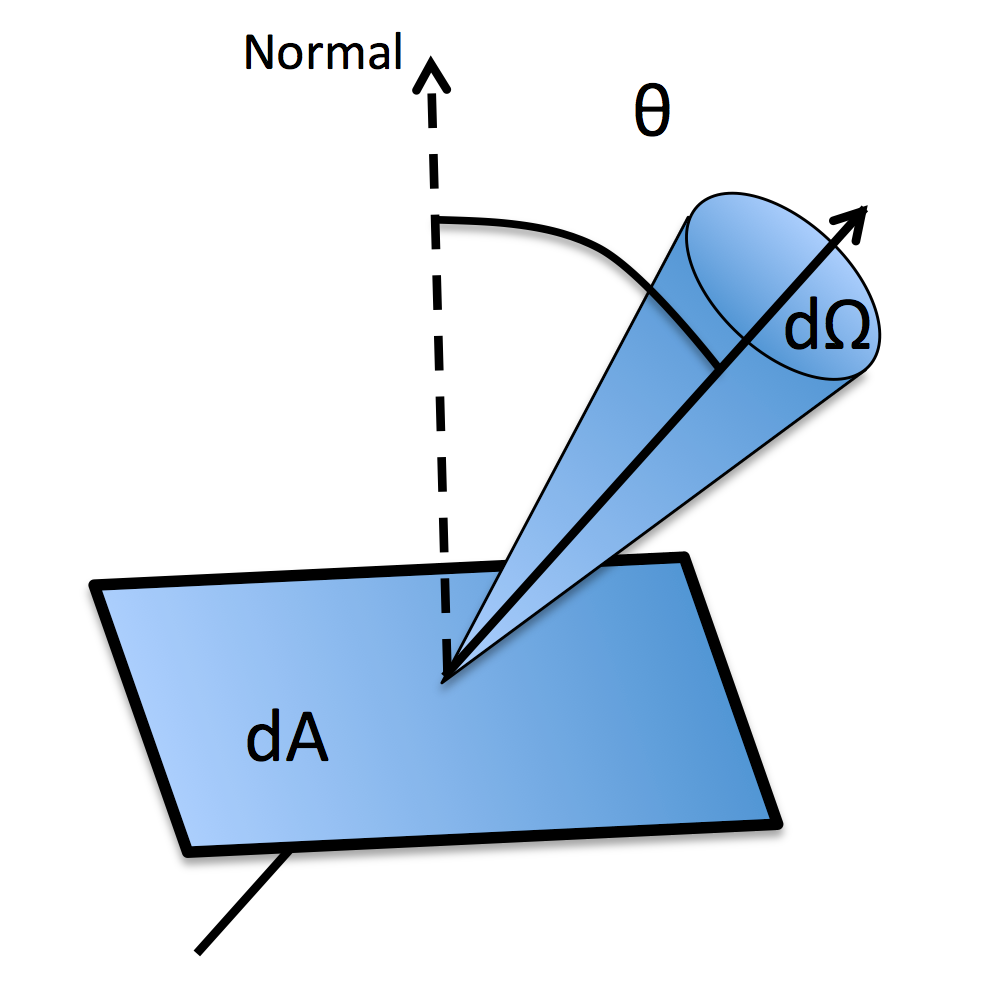
\includegraphics[width=0.5\textwidth]{figures/03-radtrans/rays_schematic.png}
\caption
{
A schematic showing a ray obliquely incident on a surface of area $dA$.
The labeled quantities are used in the definition of specific intensity.
} 
\label{fig:ray}
\end{figure}


The most fundamental quantity of radiative transfer is the 
{\em specific intensity}, $I_\nu$, defined as

\begin{equation}
I_\nu = \frac{dE}{d\Omega~dt~dA~d\nu},
\end{equation}

which has units of ${\rm erg~s^{-1}~Hz^{-1}~sr^{-1}~cm^{-2}}$.
By successively multiplying by $\cos \theta$ and integrating over solid angle we 
can obtain the first and second `moments' of the radiation field. These
are the flux, $F_\nu$ and momentum flux, $p_\nu$, respectively, given by

\begin{equation}
F_\nu = \int I_\nu \cos \theta~d \Omega,
\end{equation}

\begin{equation}
p_\nu = \frac{1}{c} \int I_\nu \cos^2 \theta~d \Omega
\end{equation}

We can also define the {\em mean intensity}, $J_\nu$, as

\begin{equation}
J_\nu = \frac{1}{4 \pi} \int I_\nu~d \Omega
\end{equation}

The mean intensity is particularly
useful when one wants to ignore the solid angle dependence of the radiation,
for example when considering the impact of an ionizing radiation field.

The equation describing the specific intensity change along a path element $ds$
is the radiative transfer equation, 

\begin{equation}
\frac{d I_\nu}{ds} = -\kappa_\nu I_\nu + j_\nu, 
\end{equation}

where $\kappa_\nu$ and $j_\nu$ are the absorption and emission coefficients respectively.
If we define the optical depth $d \tau_\nu = \kappa_\nu ds$ we can recast this as

\begin{equation}
\frac{d I_\nu}{d \tau_\nu} = -I_\nu + S_\nu
\label{eq:formal_rte}
\end{equation}

where $S_\nu=j_\nu/\kappa_\nu$ is the source function. This equation
is called the {\em formal radiative transfer equation}, and can be solved to give 

\begin{equation}
I_\nu = I_{\nu,0}~e^{-\tau_\nu} + \int^{\tau_\nu}_0 S_\nu (\tau^\prime_\nu)~e^{\tau^\prime_\nu-\tau_\nu} d \tau^\prime_\nu.
\label{eq:rte_solution}
\end{equation}

A useful limit is when the source function is constant in the absorbing medium, in which case
the integral can be easily evaluated to give

\begin{equation}
I_\nu = I_{\nu,0}~e^{-\tau_\nu} + S_\nu (1 - e^{-\tau_\nu}).
\label{eq:rte_solution}
\end{equation}

% The mean intensity, $J_\nu$ is a particularly useful quantity when calculation the ionization
% state 



\subsection{Spectral Line Formation}

From the above equations, it is trivial to show how emission and absorption lines form when
the source function is approximately constant.
Say we have a plasma illuminated by a blackbody of temperature $T_0$, such that
$I_{\nu,0} = B_\nu (T_0)$. The plasma layer then has a different temperature, $T$,
such that $S_\nu = B_\nu (T)$ in that medium. By inspecting equation~\ref{eq:rte_solution}
we can see that if we are optically thick within the line, but optically
thin in the continuum, then inside the line the source term is dominant and outside 
the line the first $I_{\nu,0}~e^{-\tau_\nu}$ term dominates. Therefore, if $T > T_0$ we will 
see an emission line, and if $T < T_0$ we will see an absorption line. 
This approach describes line emission in the blackbody limit; for more complicated SED shapes
it is necessary to construct simple model atoms.

\subsection{Local thermodynamic equilibrium}
\label{sec:lte}


An important physical limit is that of local thermodynamic equilibrium (LTE).
This is a first-order way to describe the physical conditions of a plasma, and assumes
that all the properties of the plasma, such as the level populations and source function,
are the same as those in thermodynamic equilibrium for local values of 
temperature and density. For this to be the case, the principle of 
{\em detailed balance} must also apply, in which every 
process by which electrons transition in state must be exactly 
balanced by its inverse process. LTE also assumes that $T_e = T_R$, and that
the source function is given by a blackbody, i.e. $S_\nu = B_\nu (T_R)$.
Three {\em microscopic} 
requirements of LTE also follow \citep{mihalas}:

a) The velocities of the electrons and ions in the plasma obey Maxwellian
distributions, such that
\begin{equation}
f(v) = 4 \pi \left( \frac{m}{2 \pi kT} \right)^{3/2} v^2 
\exp \left( - \frac{mv^2}{2kT} \right)
\label{eq:maxwellian}
\end{equation}

\smallskip

b) the ionization state of the plasma is governed by the {\em Saha equation},
which states that two adjacent ions have relative populations given by
\begin{equation}
\frac{N_{i+1}n_e}{N_i} = \frac{2g_{i+1}}{g_i} 
\left( \frac{2 \pi m_e kT}{h^2} \right)^{3/2}
\exp(-h \nu_0/kT)
\label{eq:saha}
\end{equation}

\smallskip

c) the excitation state of the plasma is governed by {\em Boltzmann statistics}.
Two adjacent levels then have relative populations given by
\begin{equation}
\frac{n_{j}}{n_i} = \frac{g_j}{z_i(T_R)} \exp(-E_j/kT_R), 
\label{eq:boltzmann}
\end{equation}

\smallskip

Although these three assumptions are often valid, in most astrophysical situations
there can be large departures from LTE. A good example of these departures is when
the SED is not a blackbody and is affected by absorption -- 
as is the case in AGN and other accreting systems. The Maxwellian assumption 
is probably the most reliable, but even this may break down
when high-energy photons create suprathermal electron distributions 
\citep{humphrey2014}. 

\subsubsection{Dilute approximation}
\label{sec:dilute}
A first step away from LTE is to introduce the dilute approximation. In this case,
we relax the assumption that $T_R = T_e$, and assume that the mean intensity is given
by a dilute blackbody, i.e. 
\begin{equation}
J_\nu = W B_\nu (T_R),
\label{eq:dilute_jnu}
\end{equation}
where $W$ is the dilution factor. We can then approximate the ionization state
with a modified Saha equation \citep{AL85,ML93},
\begin{equation}
\frac{N_{i+1} n_e}{N_i} = W [\xi + W(1-\xi)]
\left(\frac{T_e}{T_R}\right)^{1/2}
\left(\frac{N_{i+1}n_e}{N_i}\right)^*_{T_R}, \label{eq:ml93}
\end{equation}
where $\xi$ is the fraction of recombinations that go directly to
the ground state.
The excitation state can be approximated with a dilute Boltzmann equation \citep{lucy1999sn}
\begin{equation}
\frac{n_{ij}}{n_i} = \frac{W g_j}{z_i(T_R)} \exp(-E_j/kT_R), 
\label{eq:dilute_boltzmann}
\end{equation}
where $n_{ij}$ is the population of level $j$ in ionic stage $i$,
$E_j$ is the energy difference between level $j$ and the ground state,
$g_j$ is the statistical weight of level $j$
and $z_i(T_R)$ is the partition function of ionic stage $i$. 

\subsection{The Two Level Atom and Escape Probabilities}

The two level atom formalism is well described by \cite{mihalas}.
Let us consider an atomic model consisting of two levels that are linked 
by radiative and collisional transitions, that can also interact with the 
continuum. Whilst this model is clearly a simplification, it nonetheless allows
for a first step into non-LTE line transfer and proves useful for modelling
the resonance lines briefly touched on in chapter 2.

To construct our simple model we must make a few assumptions. The first
is the assumption of {\em statistical equilibrium}. This is the principle 
that the total rate into a given atomic level/state is equal to the 
total rate out of said state. This is clearly true whenever the timescale
to establish this equilibrium is shorter than the timescale on which
the ambient conditions change. The second is the assumption of
{\em complete redistribution (CRD)}, which states that the emission
and absorption line profiles are identical for a given transition. This 
assumption is somewhat analogous to the Sobolev approximation 
(see section~\ref{sec:sobolev}). 
These assumptions allow us to formulate rate equations and derive the 
Einstein relations.

\subsubsection{Einstein coefficients}

Within a two level atom, the rate equation between the two levels in LTE can
can be written by invoking detailed balance, such that 
\begin{equation}
B_{lu} \bar{J}_{ul} n_l = B_{ul} \bar{J}_{ul} n_u + A_{ul} n_u,
\label{eq:rate_einstein}
\end{equation}
where $B_{ul}$, $B_{ul}$ and $A_{ul}$ are the {\em Einstein coefficients}
for absorption, stimulated emission and spontaneous emission respectively.
The `mean intensity in the line', $\bar{J}_{ul}$, is given by
\begin{equation}
\bar{J}_{ul} = \int \phi(\nu) J_\nu d\nu.
\label{eq:jbar}
\end{equation}
We can then rearrange equation~\ref{eq:rate_einstein} in terms of 
the mean intensity, giving
\begin{equation}
\bar{J}_{ul} = \frac{A_{ul} / B_{ul}}{(n_l/n_u)(B_{ul}/B_{lu}) - 1}.
\label{eq:jbar2}
\end{equation}
In LTE, $\bar{J}_{ul} = B_\nu (T)$ and the level populations obey Boltzmann statistics, so we can combine equations~\ref{eq:planck}, \ref{eq:boltzmann}
and \ref{eq:jbar2} to write
\begin{equation}
\frac{2 h \nu^3}{c^2} \frac{1}{\exp(h\nu / kT) - 1} =
\frac{A_{ul}}{B_{ul}} \frac{1}{(g_l/g_u)(B_{ul}/B_{lu}) \exp(h\nu / kT) - 1}.
\end{equation}
This must be true at all values of $T$, so we can simply equate coefficients
to show that
\begin{eqnarray}
\frac{A_{ul}}{B_{ul}} &=& 2 h \nu_{ul}^3/c^2, \\  
\frac{B_{lu}}{B_{ul}} &=& g_u/g_l.  
 \label{eq:einstein_relations}     
\end{eqnarray}
These two equations are known as the {\em Einstein relations}, and have 
no dependence on temperature. They are therefore purely atomic properties.

\subsection{The Sobolev Approximation}
\label{sec:sobolev}
The Sobolev approximation (SA) is a useful limit 
used to treat line transfer in fast-moving flows. Originally 
the theory was mostly applied to stellar winds, although since then
a wide variety of astrophysical objects have been modelled using Sobolev treatments,
such as accreting systems (this work) and supernovae.

The Sobolev limit is when the local bulk velocity gradients in a flow 
dominate other any thermal broadening. In the presence of these steep
velocity gradients, one can assume that the interaction of a ray with a bound-bound
transition takes place over a small resonant zone, known as a 
`Sobolev surface'. The length of this zone is defined by
\begin{equation}
l_s = \frac{v_{th}}{dv / ds}.
\end{equation}
It is important that the physical conditions of the c do not change on this scale.
If this is the case, then we can assume that all line interactions for a given 
frequency will occur at a single `resonant' point. The location at which
a given photon will interact with a line of frequency $\nu_{lu}$
is then given, in velocity space, by
\begin{equation}
v = c~\left(\frac{\nu}{\nu_{lu}} + 1\right).
\label{eq:resonance}
\end{equation}
The Sobolev optical depth is then
\begin{equation}
d \tau = \frac{\pi e^2}{m c}  \left(n_l - n_u \frac{g_l}{g_u} \right) \frac{f_{lu} \lambda_{lu}}{c | dv / ds |}.
\label{eq:tau_sob}
\end{equation}
We can see that the physical quantities determining line opacity are therefore 
the level populations in the plasma, the velocity gradient and the atomic physics
associated with the bound-bound transition.

\subsubsection{Two-level Atom with Escape Probabilities}

Let us now write down the rate equation linking our two-level atom,
\begin{equation}
B_{lu} \bar{J}_{ul} n_l + C_lu n_l = 
B_{ul} \bar{J}_{ul} n_u + A_{ul} n_u + C_{ul} n_u,
\label{eq:rate_2level}
\end{equation}
where we have now introduced collisional rates $C_{ul}$ and $C_{lu}$.
We now seek to find a relation between the source function
and the intensity that will simplify the coupled problem of radiative transfer
and statistical equilibrium. When we consider a two-level atom
plus continuum this can be written  as \citep{mihalas}
\begin{equation}
S = (1 - q) \bar{J}_{ul} + q B(\nu_{ul}),
\label{eq:rate_2level}
\end{equation}
where $B(\nu_{ul})$ is the Planck function at line centre.



\subsection{Monte Carlo approaches}

Simple radiation transfer problems can be solved analytically,
but with more complicated geometries it is necessary to use Monte Carlo
techniques, which are easily solved with modern computing approaches and 
are intuitively parallelisable problems. I will describe one specific 
Monte Carlo radiative transfer (MCRT) code, which has been used
for the majority of the work in this thesis.









%%%%%%%%%%%%%%%%%%%%%%%%%%%%%
% PYTHON
%%%%%%%%%%%%%%%%%%%%%%%%%%%%%

\section{{\sc python}: A Monte Carlo Ionization and Radiative Transfer Code}
\label{sec:python}

\py\footnote{Named c. 1995, predating the inexorable rise of a certain widely used
programming language.} is a confusingly named 
Monte Carlo ionization and radiative transfer code. 
The general philosophy of the code is to be able to produce synthetic spectra
for astrophysical objects with outflows in 2.5D, using a self-consistent ionization 
treatment. The code is written in C, and has been in development since the mid-1990s.
Throughout this time it has been used with application to CVs \citep{LK02, M15},
YSOs \citep{simmacro2005}, supernovae \citep{kerzendorfsim} and AGN/quasars 
\citep{higginbottom2013,H14,M16}. It is also capable of producing spectra 
for stellar winds and conducting simple photoionization balance calculations for
comparison with codes such as \textsc{cloudy}. Some more detail on code testing and 
development can be found in sections~\ref{sec:code_validation} and \ref{sec:code_maintenance}
respectively. Although the operation of \py\ is well-described by the above authors,
it is central to this Thesis and I will thus provide substantial detail on its operation. 

\subsection{Basics}

\begin{figure}
\centering
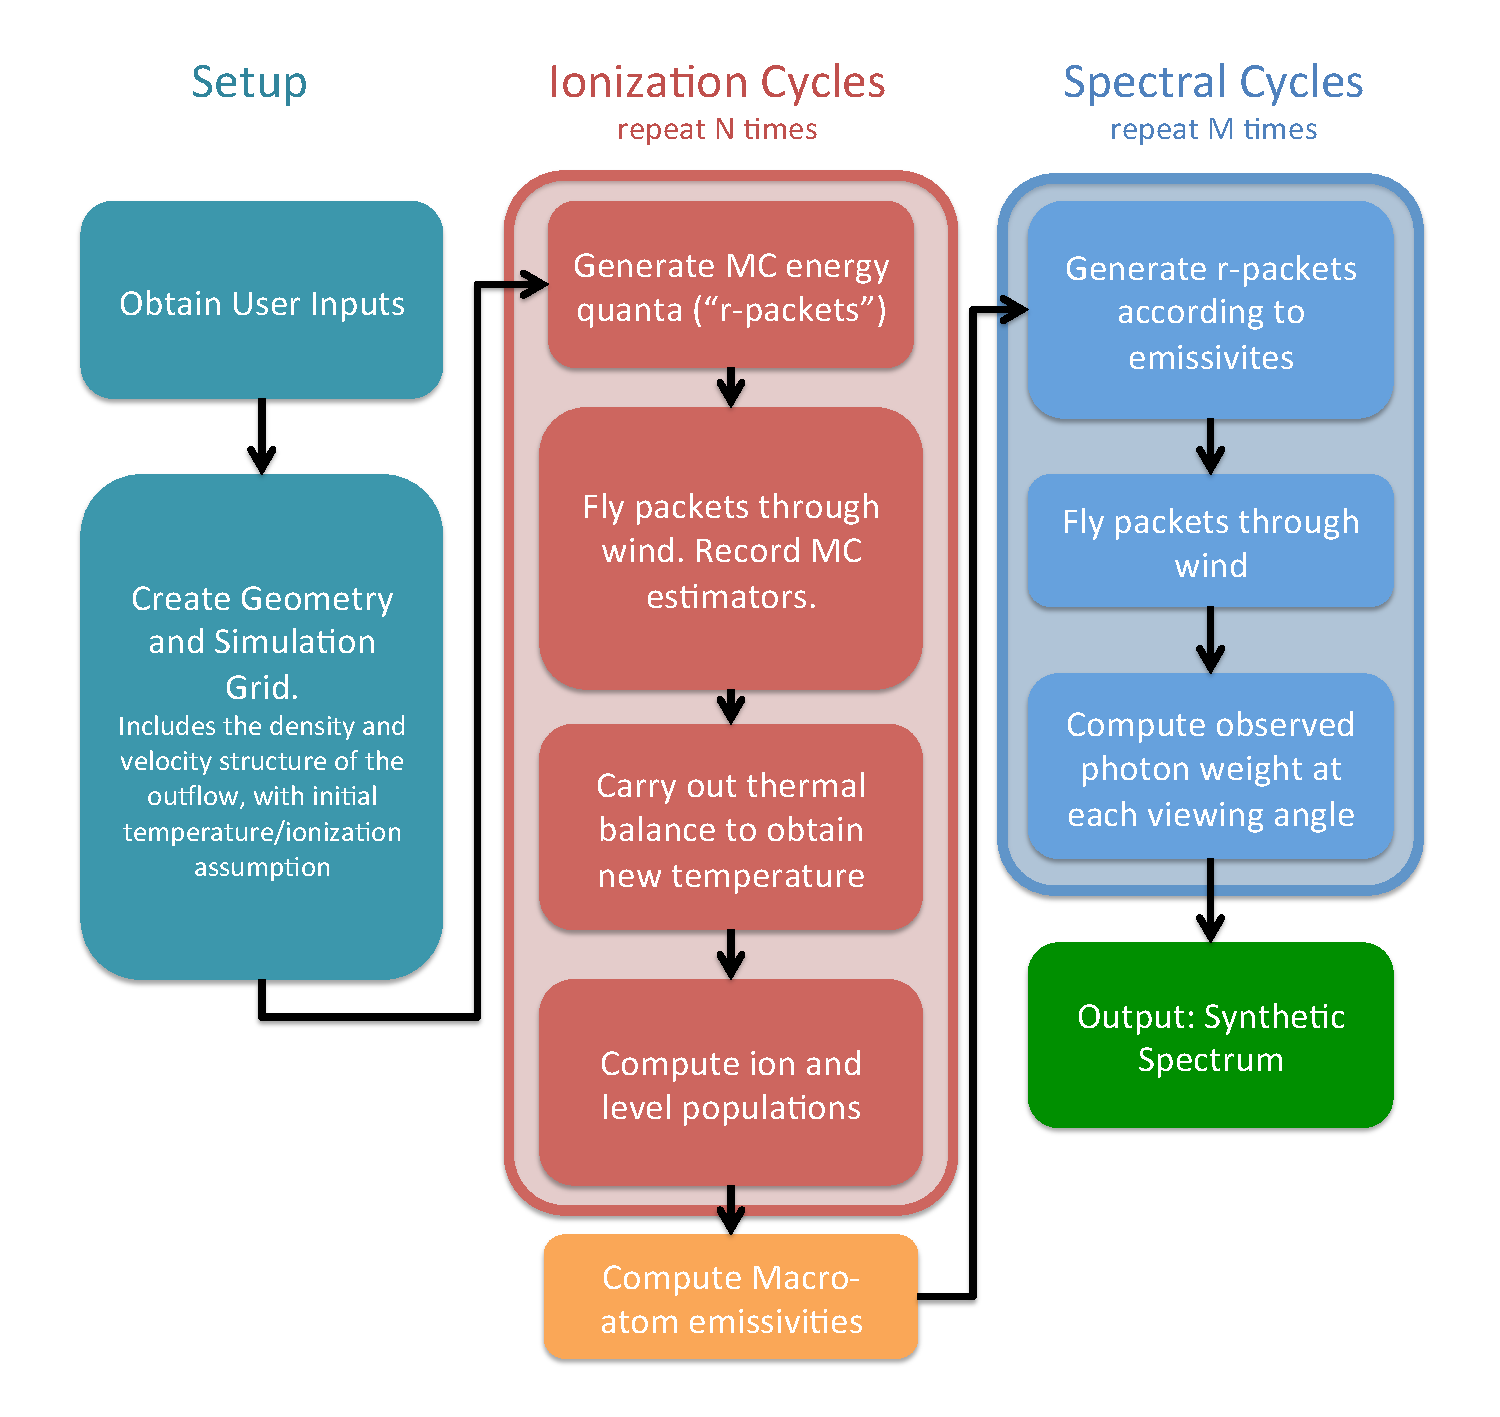
\includegraphics[width=1.0\textwidth]{figures/03-radtrans/flowchart.pdf}
\caption
{
A flowchart showing the basic operation of \py.
} 
\label{fig:flowchart}
\end{figure}

\py\ operates in three distinct stages, shown in figure~\ref{fig:flowchart}. 
First, the user specifies the photon sources,
geometry and kinematics of the system, normally with a similar parameterisation
to the SV93 model described in section~\ref{sec:sv93_model}. 
The code can operate with multiple coordinate systems 
(1D, spherical polar, cylindrical), but in this work I use cylindrical coordinates.
In this case, the outflow is discretised into a $n_x \times n_y$ logarithmic grid with 
user-specified dimensions. The co-ordinates, $(x_i, z_i$), 
of the corner of the $i$th cell are then given by
\begin{align}
x_i &= L_{x}~10^{(i-1)\frac{\log (R_{max} / L_{x})}{n_x}},\\
z_i &= L_{z}~10^{(i-1)\frac{\log (R_{max} / L_{z})}{n_z}},
\end{align}
where $L_x$ and $L_z$ are appropriately chosen (but hardwired) scale lengths.
From these co-ordinates the poloidal distance can be calculated and
the velocity set according to equation~\ref{eq:v_law}. The density
is then calculated from equation~\ref{eq:rho_rz}. An initial temperature,
$T_{init}$ is set by the user. The ionization fractions throughout
the wind are then to Saha (LTE) abundances at $T_{init}$, and the level 
populations are set according to the Boltzmann formula.

Once the basic setup process has been carried out, the ionization state,
level populations and temperature structure are calculated.
This is done via an iterative process, by transporting several populations of 
Monte Carlo energy quanta (`photons' or `$r$-packets) through the outflow.
This process is repeated until the code converges. 
In each of these iterations (`ionization cycles'), the code records estimators that 
characterize the radiation field in each grid cell. At the end 
of each ionization cycle, a new electron temperature is calculated
that more closely balances heating and cooling in the 
plasma. The radiative estimators and updated electron
temperature are then used to revise the ionization state of the wind,
and a new ionization cycle is started. The process is repeated until
heating and cooling are balanced throughout the wind. 

This converged model as the basis for the second set of
iterations (`spectral cycles'), in order to compute the synthetic spectrum based on the 
MC estimators record during the ionization cycles. 
The emergent spectrum over the desired spectral range is synthesized by 
tracking populations of energy packets through the wind and computing the emergent spectra at
a number of user-specified viewing angles.  

% \py\ is designed to operate in a number of different
% regimes, both in terms of the scale of the system and in terms of the
% characteristics of the underlying radiation field.
% It was originally developed by LK02 in order to model the UV spectra
% of CVs with a simple biconical disc wind model. SDL05
% \nocite{simmacro2005} used the code to model Brackett
% and Pfund line profiles of H in young-stellar objects (YSOs). As part
% of this effort, they implemented a `macro-atom' mode (see below) in
% order to correctly treat H recombination lines with
% \py. Finally, H13 used \py\ to model broad absorption line (BAL) QSOs. For
% this application, an improved treatment of ionization was implemented,
% so that the code is now capable of dealing with arbitrary
% photo-ionizing SEDs, including non-thermal and multi-component ones. 
\subsection{Radiation Packets}
\label{sec:packets}
Every energy packet in the simulation starts out as a radiation packet generated
from one of $N_S$ photon sources. To ensure that the frequency distribution
of photons is adequately sampled in important frequency regimes, 
{\em stratified sampling} is used. A specified fraction, $f_i$,
of photons must then emerge each band $i$, whose frequency boundaries
can be adapted for the astrophysical situation considered. 
The weight, $w_i$, of the radiation packets in a given energy band $i$, with boundaries
$\nu_i$ and $\nu_{i+1}$ is then given by
\begin{equation}
w_i = \frac{\sum_j^{N_S} \int_{\nu_i}^{\nu_{i+1}} L_{\nu,j}~d\nu}{f_i~N_p},
\end{equation}
where $N_p$ is the {\em total} number of photons desired 
and $L_{\nu,j}$ is the monochromatic 
luminosity of photon source $j$. 
The frequency of photons is calculated by constructing a 
cumulative distribution function (CDF), $f_{C,i}(\nu)$
from the spectral energy distribution in each band $i$: 
\begin{equation}
f_{C,i} (\nu) = 
\frac{\int_{\nu_i}^{\nu} L_\nu~d\nu}
{\int_{\nu_i}^{\nu_{i+1}} L_\nu~d\nu} ~.
\end{equation}
A photon frequency can then be generated by cycling through the bands. In each band,
a random number is chosen between 0 and 1, and then the frequency is 
selected by interpolating on the sampled CDF. This process is repeated until 
each band has the specified number of photons, with the packet
weights adjusted accordingly.

\py\ can operate in two modes concerning the approach to energy packets. 
In the original mode described by LK02, continuum processes attenuate 
the weight of the radiation packets. This attenuation is accounted for 
by including the wind as an additional photon source.
In the second mode, energy packets are indivisible and strict radiative equilibrium is
enforced. From here on I will only be discussing this indivisible packet scheme, 
as it is required in order to be able to use macro-atoms to accurately
treat recombination in H and He.

\subsection{Radiative Transfer procedure}

As a photon travels through a plasma, it has a finite probability
of interacting with the free or bound electrons and undergoing a scattering
or absorption event. To deal with this in a Monte Carlo sense, a random optical 
depth is generated before an $r$-packet is moved,
\begin{equation}
\tau_R = - \ln (1 - {\cal Z}),
\end{equation}
where ${\cal Z}$ is a random number between 0 and 1. 
The $r$-packet is then gradually transported through a given cell. 
As it moves, the optical depth, $\tau^\prime$, it experiences
is incremented continuously, representing continuum processes. When the $r$-packet comes
into resonance with a line, according to equation~\ref{eq:resonance}, then
the Sobolev optical depth is calculated from equation~\ref{eq:tau_sob} and added to 
$\tau^\prime$. This process is shown in Fig.~\ref{fig:scatter_ml93}, and
continues until $\tau^\prime \geq \tau_R$ or the $r$-packet leaves the cell. If the
photon leaves the cell then the values of $\tau_R$ and $\tau^\prime$ are preserved,
and the process continues using the conditions in the new cell. If 
$\tau^\prime \geq \tau_R$, then an interaction with the plasma has occurred, and
the process governing this interaction must be identified. This is done by
randomly picking an interaction process in proportion with their contributions
to $\tau^\prime$. If the process is an electron scatter then a new, isotropic
direction is generated for the $r$-packet. Otherwise, the packet must
interact with either the thermal pool or the excitation energy of the plasma.

\begin{figure}
\centering
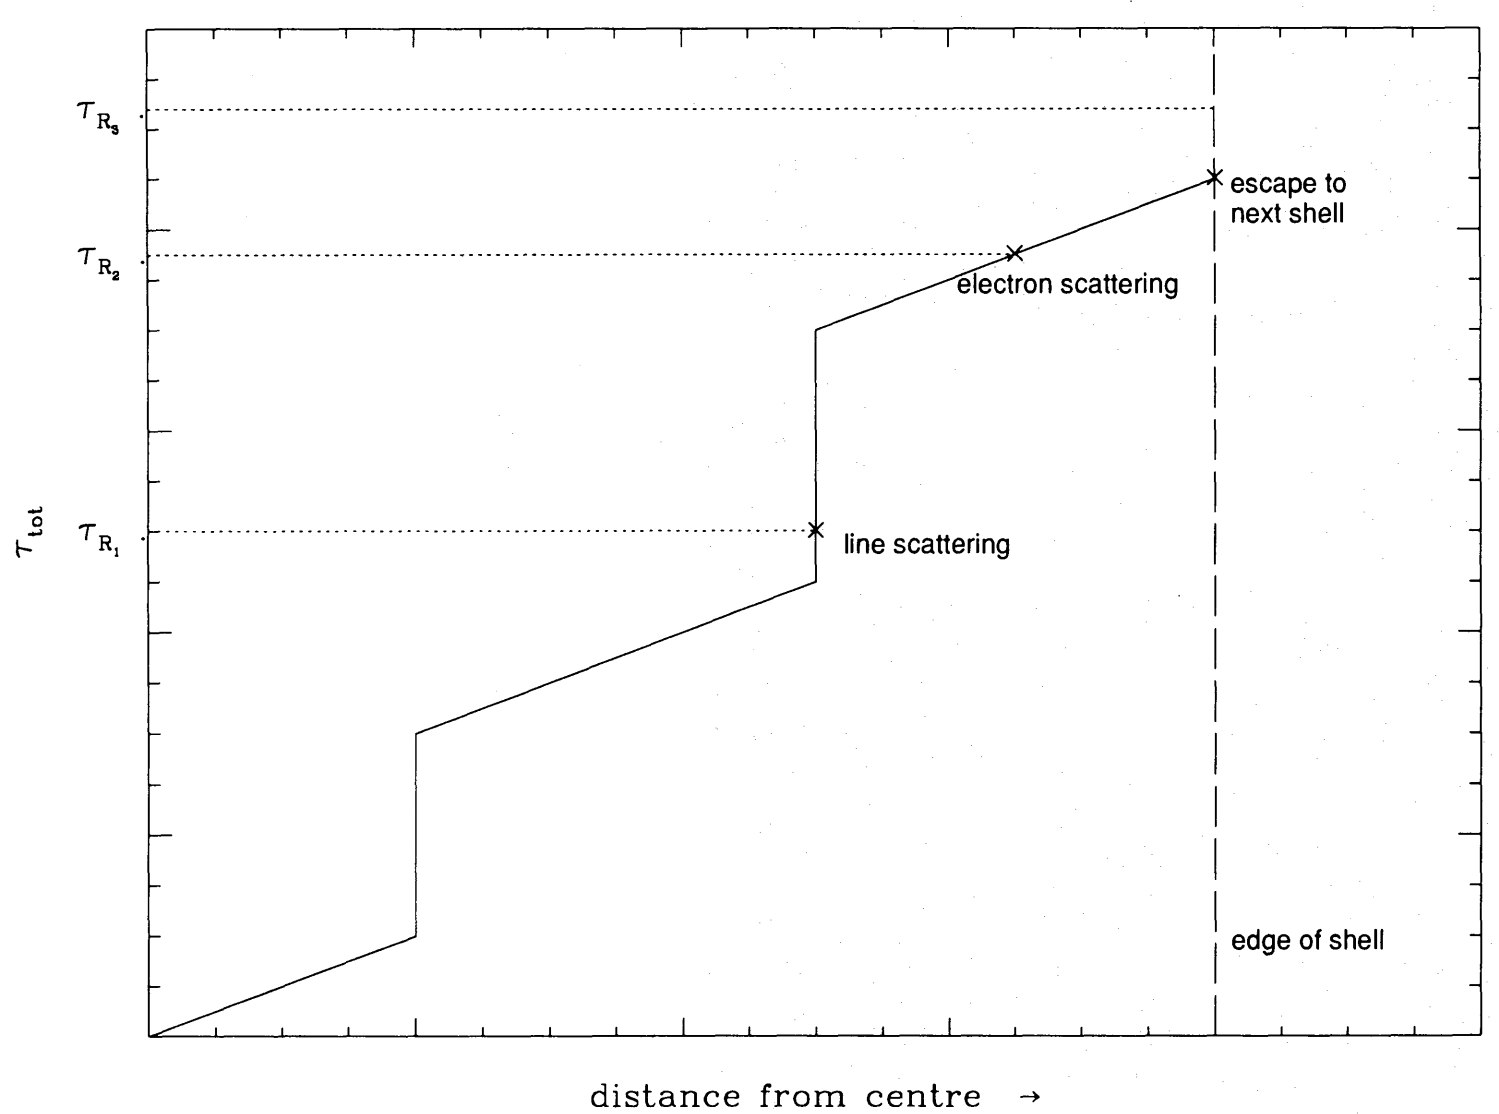
\includegraphics[width=0.7\textwidth]{figures/03-radtrans/tau_scat.png}
\caption
{
{\sl Credit: Mazzali \& Lucy 1993}. 
The process of choosing a scattering location in a cell.
} 
\label{fig:scatter_ml93}
\end{figure}

\subsubsection{Continuum opacities}

In order to calculate $\tau^\prime$ in the above approach, we need
to know the opacities that will contribute to it. An opacity 
at a given frequency, $\kappa(\nu)$,
is related to an optical depth, $\tau(\nu)$, by
\begin{equation}
\tau(\nu) = \kappa(\nu)~\Delta s,
\end{equation}
where $\Delta s$ is the distance moved by the photon. The bound-free
opacity is calculated from a sum over photoionization cross-section,
such that
\begin{equation}
\kappa_{bf} = .
\end{equation}
The free-free emission coefficient for an individual ion $i$ is \citep{gayet1970}
\begin{equation}
j_{ff,i} (\nu) = \bar{g}_{ff}\frac{8Z_i^2e^6}{3m_e c^2}
\frac{2\pi m_e}{3 k T_e}^{1/2}
N_i n_e \exp(-h\nu/kT_e).
\label{eq:jff} 
\end{equation}
The free-free opacity is then calculated from Kirchhoff's law, 
\begin{equation}
\kappa_{ff, i}(\nu) = \frac{B_\nu (T_e)}{j_{ff,i} (\nu)},
\end{equation}
which gives
\begin{equation}
\kappa_{ff, i}(\nu) = n_e N_i \frac{4}{3} \left(\frac{2\pi}{3}\right)^{1/2} 
\frac{Z_i^2}{e^6 m_e^2 hc} \left(\frac{m_e}{kT_e}\right)^{1/2} 
g_{ff} \nu^{-3} [1 - \exp(-h\nu/kT_e)].
\end{equation}
The electron scattering opacity is then 
\begin{equation}
\kappa_{es} = \sigma_T n_e \Delta s.
\end{equation}
These opacities are all used in the heating and cooling estimators 
introduced in section~\ref{sec:estimators}. In addition the
Compton opacity is required in order to estimate the Compton heating effect on the plasma.
The Compton opacity is given by
\begin{equation}
\kappa_{C} = ,
\end{equation}
where $\sigma_KN (\nu)$ is the cross-section computed 
from the Klein-Nishina formula \citep{klein-nishina}, and unliked $\sigma_T$
is frequency dependent. This opacity is not included in the actual radiative transfer 
in the simulations presented in this Thesis.

\subsubsection{Doppler Shifts}

To calculate the opacities correctly, the frequency must be shifted from
the co-moving frame of the photon into the co-moving frame of the cell.
This is done...




\subsubsection{Choosing packet directions}

The initial directions from the photon sources are chosen
depending on an angular emissivity function, $\eta(\theta)$.


Whenever a radiation packet undergoes an electron scatter,
the new direction is simply chosen to be isotropic. However,
when the photon is a line photon then the new direction is chosen
according to a line trapping model, which depends on the Sobolev
optical depths in different directions. 





%%%%%%%%%%%%%%%%%%%%%%%%%%%%%
%%%%%%%%%%%%%%%%%%%%%%%%%%%%%
% MACRO ATOMS
%%%%%%%%%%%%%%%%%%%%%%%%%%%%%
%%%%%%%%%%%%%%%%%%%%%%%%%%%%%

\section{Macro-atoms}

{\sl The macro-atom scheme was created by Leon Lucy and is outlined in 
his 2002/03 papers. It was implemented in \py\ by Stuart Sim, initially
for the study of recombination lines in YSOs \citep{simmacro2005}
}

\cite{lucy2002, lucy2003}
has shown that it is possible to calculate the emissivity of a gas in
statistical equilibrium without approximation for problems with large departures
from LTE.
% accurately by quantising matter into
% `macro-atoms', and radiant and kinetic energy into indivisible energy
% packets (r- and k- packets, respectively). 
His macro-atom scheme allows for all possible transition paths from a given level,
dispensing with the two-level approximation, and
provides a full non-LTE solution
for the level populations based on Monte Carlo estimators. The macro-atom
technique has already been used to model Wolf-Rayet star
winds \citep{sim2004}, AGN disc winds \citep{simlong2008, tatum2012},
supernovae \citep{kromersim2009, kerzendorfsim} and YSOs (SDL05). A full 
description of the approach can be found in L02 and L03. 

The fundamental approach here requires somewhat of a philosophical shift.
Normally MCRT is described in the most intuitive way- that is, we imagine
real photons striking atoms and scattering, or photoionizing 
and depositing energy in a plasma. With Lucy's scheme we should instead 
reimagine the MC quanta as a packets of quantised energy flow, and the scheme as a 
{\em statistical} one. The amount of time a given energy quanta spends in a specific atomic
level or thermal pool is then somewhat analogous to the absolute energy 
contained therein.

Following L02, let us consider an atomic species interacting with a radiation field.
If the quantity $\epsilon_j$ represents the ionization plus excitation energy of 
a level i then the rates at which the level $j$ absorbs and emits radiant energy 
are given by
\begin{equation}
 \dot{A}_{j}^{R} = R_{\ell j} \epsilon_{j \ellp} \;\;\;\;\; {\rm and} \;\;\;
\;\;  \dot{E}_{i}^{R} = R_{j \ellp} \epsilon_{j \ellp} \;\;\; ,
\end{equation}
Where I have adopted Lucy's convention in which the subscript 
$\ellp$ denotes a summation over all lower states ($\ellp<j$), and
$\up$ will thus denote a summation over all states ($\up>j$).
Similarly, the rates corresponding to {\em kinetic} (collisional)
energy transport can then be written as
\begin{equation}
 \dot{A}_{j}^{C} = C_{\ellp j} \epsilon_{j \ellp} \;\;\;\;\; {\rm and}
\;\;\;
\;\;  \dot{E}_{j}^{C} = C_{j \ellp} \epsilon_{j \ellp} \;\;\; ,
\end{equation}
If we now impose statistical equilibrium
%
\begin{equation}
 ({\cal R}_{\ellp j}-{\cal R}_{j \ell})+({\cal R}_{uj}-{\cal R}_{ju})=0 \;\;\;.
\end{equation}
we can then obtain 
\begin{eqnarray}
 \dot{E}_{j}^{R}+\dot{E}_{j}^{C}+{\cal R}_{j\up}\epsilon_{j}+
 {\cal R}_{j \ell}\epsilon_{\ellp}  \nonumber \\  
 = \dot{A}_{j}^{R}+\dot{A}_{j}^{C}+{\cal R}_{\up j} \epsilon_{j}
 +{\cal R}_{\ellp j} \epsilon_{\ellp}           .  
 \label{eq:matom_SE}     
\end{eqnarray}
This equation is the starting point for the macro-atom scheme. It shows 
that, when assuming only radiative equilibrium, the energy flows through
a system depend only on the transition probabilities and atomic physics
associated with the levels the energy flow interacts with.
By quantising this energy flow into radiant ($r$-) and kinetic ($k$-) packets, 
we can simulate the energy transport through
a plasma discretised into volume elements (``macro-atoms''),
whose associated transition probabilities govern the interaction 
of radiant and kinetic energy with the ionization and excitation energy associated 
with the ions of the plasma.

Although equation~\ref{eq:matom_SE} assumes strict radiative equilbrium,
it is trivial to adjust it to include non-radiative source and sink terms. 
For example, in an expanding parcel of plasma, adiabatic cooling may be 
included with a simple modification to the RHS of equation~\ref{eq:matom_SE}.


%%%%%%%%%%%%%%%%%%%%%%%%%%%%%
% PROBS
%%%%%%%%%%%%%%%%%%%%%%%%%%%%%

\subsection{Transition Probabilities}

Having interpreted equation~\ref{eq:matom_SE} in a {\em stochastic} way,
we can now construct our Monte Carlo scheme, following \cite{lucy2002}.
A macro-atom in state $j$ always has a finite probability of deactivating
radiatively or collisionally:
\begin{equation}
p_{j}^{R} = \dot{E}_{j}^{R} / D_j \;\;\;\;\; {\rm and} \;\;\;
\;\; p_{j}^{C} = \dot{E}_{j}^{C} / D_j,
\label{eq:deactivate}
\end{equation}
where I have defined
\begin{equation}
D_j =  \dot{E}_{j}^{R}+\dot{E}_{j}^{C}+{\cal R}_{j\up}\epsilon_{j}+
 {\cal R}_{j \ellp}\epsilon_{\ellp} = ({\cal R}_{j\ellp} + {\cal R}_{j\up}) \epsilon_{j}.
\end{equation}
The corresponding jumping probabilities, which describe the probability
that the macro-atom transitions to a different state while remaining active, 
are given by
\begin{equation}
p_{j\up} = {\cal R}_{ju} \epsilon_{j} / D_j \;\;\;\;\; {\rm and} \;\;\;
\;\; p_{j\ellp} = {\cal R}_{j\ellp} \epsilon_{\ellp} / D_j.
\end{equation}
Note that the jumping probability is always proportional to the energy
of the lower level, whereas the emission probability is proportional
to the energy {\em difference} between the levels, as 
$\dot{E}_{j}^{R} = R_{j\ellp} (\epsilon_j - \epsilon_\ellp)$. We can also
trivially show that the probabilities are correctly normalised, as
\begin{align}
p_{j}^{R} + p_{j}^{C} + p_{j\ellp} + p_{j\up} &=
(1/D_j) ( {\cal R}_{j\up} \epsilon_{j} + {\cal R}_{j\ellp} \epsilon_{\ellp} +
\dot{E}_{j}^{R} + \dot{E}_{j}^{C}) \\
&= 1. \nonumber
\end{align}

With these transition
probabilities identified, a Monte Carlo calculation can proceed by formulating
the normal statistical equilibrium rate equations that will depend on
the ambient conditions of the plasma. The effect of these ambient conditions
is expressed through the use of Monte Carlo {\em estimators}.




%%%%%%%%%%%%%%%%%%%%%%%%%%%%%
% RATES
%%%%%%%%%%%%%%%%%%%%%%%%%%%%%
\subsection{Rate equations}

The macroscopic transition probabilities above depend on the traditional
rate equations formulated according to statistical equilibrium. 
In the framework of the Sobolev escape probability formalism 
(Rybicki \& Hummer 1978; L02; Sim 2004), 
the bound-bound excitation rate, ${\cal R}_{lu}$, in an ion is given by 
\begin{equation}
{\cal R}_{ju} = B_{ju} n_j J_{est} + q_{ju} n_j n_e,
\label{eq:rad_rate}
\end{equation}
where $u$ is now a specific upper level and $q_{ju}$ is the collisional
rate coefficient (see section~\ref{sec:coll}).
$J_{est}$ is the Monte Carlo estimator for the mean intensity 
impinging on the Sobolev region, weighted by an angle-dependent escape probability, 
given by \citep{sim2004}
\begin{equation}
J_{est} = \frac{c}{4 \pi \nu_0 V} \sum_{i} w_i \frac{1 - e^{-\tau_{s,i}}}{\tau_{s,i}} \frac{1}{(dv/ds)_i}.
\end{equation}
Here $w$ is the photon weight (in luminosity units), $\nu_0$
is the line frequency, $dv/ds$ is the velocity gradient and
$\tau_s$ is the Sobolev optical depth.
The sum is over all photons that come into resonance with the line,
and thus represents an integral over solid angle.
This is essentially the MC estimator form of $\bar{J}_{ul}$, and differs
from the $J^b_{ji}$ quantity in equation~(20) of \cite{lucy2002} as 
there is no assumption of homologous flow or symmetric escape probabilities.
The corresponding de-excitation rate is then 
\begin{equation}
{\cal R}_{uj} = \beta_{ju} A_{uj} n_u + B_{uj} n_u J_{est} +
q_{uj} n_u n_e.
\label{eq:nlte_rul}
\end{equation}

The photoionization and collisional ionization rates
between a lower level, $l$, and the continuum level $\kappa$ 
(or, in the case of ions with more than one bound electron, 
the ground state of the upper ion),
$\kappa$, are
\begin{equation}
{\cal R}_{j \kappa}= n_j (\gamma_{j\kappa} - \alpha^{st}_{\kappa j})  + q_{j \kappa} n_j n_e.
\end{equation}
Here, $q_{j \kappa}$ is the collisional ionization rate coefficient, 
$\gamma_{j \kappa}$ is the photoionization rate
from $j \rightarrow \kappa$ and $\alpha^{st}_{\kappa j}$ is the stimulated recombination
coefficient. This is included as a negative photoionization term rather 
than a positive recombination term as in \cite{lucy2003}, which requires no
population inversions (see section ??). 
The corresponding recombination rate is given by 
\begin{equation}
{\cal R}_{\kappa j} = \alpha_{\kappa j} n_{\kappa} n_e + q_{\kappa j}
n_\kappa n_e, \\
\end{equation}
where $\alpha_{\kappa l}$ is the radiative recombination coefficient
to level $l$, and is given by 
\begin{equation}
\alpha_{\kappa j} = 4\pi \Phi^*_{j\kappa} \int^\infty_{\nu_0} 
\frac{\sigma_{j\kappa} (\nu)}{h \nu} \frac{2 h \nu^3}{c^2} 
\exp \left( \frac{- h \nu}{k T_e} \right) d\nu.
\end{equation}
This treatment means that radiative and collisional
rates to and from all levels are considered when calculating both the
ionization state and the level populations, although we neglect 
ionization directly to excited levels of the upper ion. 

\subsubsection{Collision strengths}
\label{sec:coll}

The bound-bound collisional rate coefficient $q_{lu}$ is calculated from the
\cite{vanregemorter} approximation, given by
\begin{equation}
q_{ju} = 2.388 \times 10^{-6}~\lambda_{uj}^3~A_{uj}~g_u~\bar{g}
\label{eq:vanregemorter}
\end{equation}
and the inverse rate can just be calculated by considering detailed balance, 
such that
\begin{equation}
q_{uj} = q_{ju} \frac{g_u}{g_j} \exp \left( \frac{h \nu_{uj}}{k T_e} \right)
\label{eq:vanregemorterw}
\end{equation}
Using equation~\ref{eq:vanregemorter} means that collisions between radiatively
forbidden transitions are not taken into account when one 
splits levels into $l$- and $s$-subshells, as well
as principal quantum number, $n$ (as we have done with He~\textsc{i}; 
see section~\ref{sec:data}). Although this approximation is, in general, 
a poor one, the effect is second order in the physical 
regime where recombination lines are formed in our models. 
This is because bound-free processes are dominant in determining 
level populations and emissivities. We have verified that this 
is indeed the case in the He~\textsc{i} emission regions in our models.

The bound-free collision strengths are calculated using equation~(5.79) of
\cite{mihalas}. The collisional ionization rate is
\begin{equation}
q_{j\kappa} = 1.55 \times 10^{-13} n_e~\bar{g}_{i}~\sigma_{j\kappa} (\nu_0)~
\frac{h \nu_{uj}}{k T_e^{3/2}}
\exp \left( \frac{- h \nu_{\kappa j}}{k T_e} \right),
\label{eq:vanregemorterw}
\end{equation}
where $\sigma_{l\kappa} (\nu_0)$ is the photoionization cross-section 
at the threshold energy.
$\bar{g}_{i}$ is an effective gaunt factor for ion $i$ and is approximately
equal to $0.1,0.2,0.3$ for $Z=1,2$ and $>2$ respectively,
where $Z$ is the atomic number. Note that the use of this estimator
implies a $\nu^{-3}$ shape to the photoionization cross-section,
which is only strictly true for for hydrogenic ions.
The collisional (three-body) recombination rate is found using the Saha equation
and given by
\begin{equation}
q_{\kappa j} = q_{j\kappa} \frac{n_j^*}{n_e^* n_\kappa^*},
\label{eq:vanregemorterw}
\end{equation}
For numerical reasons, the above two expressions are combined in \py\ where 
possible, to avoid multiplying two exponentials together.





%%%%%%%%%%%%%%%%%%%%%%%%%%%%%
%ESTIMATORS
%%%%%%%%%%%%%%%%%%%%%%%%%%%%%
\subsection{Macro-atom estimators}
\label{sec:estimators}
To be able to solve the above rate equations and compute the transition 
probabilities, it is necessary to construct estimators for the various properties
of the radiation field that appear in said equations. This is done
by converting integrals over the radiation field into summations over 
$r$-packets passing through a cell. This represents the stochastic nature of
a MC simulation, and is by no means unique to the macro-atom formalism.
The first step is to apply the energy-density argument of \citep{lucy1999radeq},
which gives, for a time-independent code
\begin{equation}
J_\nu~d\nu = \frac{1}{4\pi}\frac{1}{V} \sum_{d\nu} w_i \Delta s.
\end{equation}
where the summations is over all photons between $(\nu, \nu+'d\nu)$. This allows
us to formulate estimators in a MC sense, rather than in integral form. 

\subsubsection{Bound-free estimators}
The estimator for the photoionization rate is 
\begin{equation}
\gamma_{j\kappa} = \frac{1}{V} \sum_i^{photons} 
\frac{w_i~\sigma_{j\kappa}({\nu})}{h \nu}~\Delta s
\end{equation}
and for the stimulated recombination rate is
\begin{equation}
\alpha_{\kappa j}^{st} = \Phi^*_{j\kappa}
\frac{1}{V} \sum_i^{photons} 
\frac{w_i~\sigma_{j\kappa}({\nu})}{h \nu}
~\exp(-h\nu/kT_e)~\Delta s,
\end{equation}
where $\sigma_{l\kappa} (\nu)$ is the photoionization cross-section for this transition.
For bound-free transitions, we define the normal photoionization and recombination
rate coefficients $\gamma$ and $\alpha$, where $\alpha$ includes
stimulated recombination as we do in the code. Note
this differs to the approach in Lucy (2003), where it is instead included as a 
negative photoionization term, hence the notation $\widetilde{\gamma}$.
We also need to define two `modified rate coefficients' which 
are the rates at which b-f transitions add and remove energy to the radiation field.
These are denoted $\gamma^E$ and $\alpha^E$, and given by

\begin{equation}
\gamma^E_{j\kappa} = \frac{1}{V} \sum_i^{photons} \frac{w_i~\sigma_{\nu_0}}{h \nu}~\Delta s 
\end{equation}

\begin{equation}
\alpha^E_{\kappa j} = 4\pi \Phi^*_{i\kappa} \int^\infty_{\nu_{\kappa j}} 
\frac{\sigma_{\kappa j}(\nu)}{h \nu_{\kappa j}} \frac{2 h \nu^3}{c^2} 
\exp \left( \frac{- h \nu}{k T_e} \right) d\nu
\end{equation}

\begin{equation}
\alpha_{\kappa j}^{st,E} = \Phi^*_{j\kappa}
\frac{1}{V} \sum_i^{photons} 
\frac{w_i~\sigma_{j\kappa}({\nu})}{h \nu}
~\exp(-h\nu/kT_e)~\Delta s
\end{equation}

The rate at which recombinations convert
thermal {\em and} ionization energy into radiant energy is then
$\alpha^E h\nu_{\kappa l} n_\kappa n_e$, where $h \nu_{\kappa l}$ is the potential of the 
b-f transition, or the energy difference between continuum $\kappa$ and 
the level $l$ we are recombining too. 
The amount of this energy which is removed from the actual thermal pool
therefore needs a quantity $\alpha h\nu_{\kappa l} n_\kappa n_e$ subtracted from it,
giving
\begin{equation}
\cc_{bf} = \sum_{bf jumps} (\alpha^E - \alpha) n_e n_{\kappa}\nu_{\kappa l} V 
\end{equation}
where here I have also included stimulated recombination as we do in the code. Note
this differs to the approach in Lucy (2003), where it is instead included as a 
negative photoionization term, hence the notation $\widetilde{\gamma}$.
For photoionizations, we write a similar expression. The rate of at which
a level $l$ absorbs energy by b-f transitions is given by $\gamma^E h\nu_{\kappa l} n_\kappa n_e$,
but the amount $\gamma h \nu_{\kappa l} n_l$ goes into ionization energy, giving 
\begin{equation}
\hh_{bf} = \sum_{bf jumps} (\gamma^E - \gamma) n_l h \nu_{\kappa l} V
\end{equation}
as the rate at which radiant energy heats the plasma via b-f transitions.

\subsubsection{Bound-bound estimators}
The heating and cooling rates for macro-atom bound-bound transitions are the rates of
collisional excitations and de-excitations
- i.e. the rate at which thermal energy is converted into
bound-bound excitation energy and vice versa.

\begin{equation}
\cc_{bb} = \sum_{lines} q_{lu} n_l n_e h \nu_{ul} V
\end{equation}

\begin{equation}
\hh_{bb} = \sum_{lines} q_{ul} n_u n_e h \nu_{ul} V
\end{equation}


\subsubsection{Other heating and cooling estimators}
Although we have now formulated the estimators required to calculate the 
transition probabilities and level populations, there are still a number of 
heating and cooling mechanisms that do not involve macro-atoms. 

The free-free cooling estimator is calculated from the emission coefficient
in equation~\ref{eq:jff} 
\begin{equation}
\cc_{ff} = V \sum_i^{ions} \int \frac{j_{ff,i}(\nu)}{4\pi} d\nu,
\end{equation}
where the integral is over all frequencies included in the simulation,
and the sum is also over all ions included in the simulation.
\begin{equation}
\hh_{ff} = \sum w_i \kappa_{ff} \Delta s
\end{equation}
Compton heating and cooling is included in the thermal balance and as
$(r\rightarrow k)$ and $(k\rightarrow r)$ transitions.
\begin{equation}
\cc_{comp} = 16 \pi \sigma_T V J \frac{k T_e}{m_e c^2},
\end{equation}
\begin{equation}
\hh_{comp} = n_e \sum \frac{h\nu}{m_e c^2} w_i \kappa_{C}\Delta s,
\end{equation}
and induced Compton heating is then given by \citep{cloudy2013}
\begin{equation}
\hh_{ind~comp} = n_e \sum \frac{J_\nu c^2}{h \nu^3} \frac{h\nu}{m_e c^2} 
w_i \kappa_{C} \Delta s,
\end{equation}
where the first $J_\nu c^2/h \nu^3$ term represents the `photon occupation number'.
The adiabatic cooling rate is derived from $PdV$ work and is given by
\begin{equation}
\cc_{a} = k T_e V (\nabla \cdot v) \left(n_e + \sum\limits_{i=1}^{ions} N_i\right),
\end{equation}
where $\nabla \cdot v$ is the divergence of the 
velocity field at the centre of the cell. The sum is over all ions 
included in the simulation.

\noindent

%%%%%%%%%%%%%%%%%%%%%%%%%%%%%
% K PACKETS
%%%%%%%%%%%%%%%%%%%%%%%%%%%%%
\subsection{$k$-packets}
$k$-packets represent quantised kinetic or thermal energy, and any interaction
chain involving a $k$-packet thus represents interaction with the thermal
pool of ions and electrons. $k$-packets can be produced either directly
via a continuum heating process ($r \rightarrow k$), 
or by the collisional de-activation of a macro-atom 
($r \ldots \rightarrow A^* \rightarrow k$) according to equation~\ref{eq:deactivate}. 

Once they are produced, $k$-packets never move, as they represent the quantised
thermal energy flow in a finite volume element. Hence, when they are produced,
their destruction path is decided according to the different cooling mechanisms
in the plasma. A $k$-packet then has a probability of being destroyed by process $i$ of
\begin{equation}
p_{i,destruct} = \cc_i / (\cc_{bf} + \cc_{ff} + \cc_{bb} + \cc_{comp} + \cc_a).
\end{equation}
Note that only adiabatic cooling leads to an actual destruction of the energy packet,
as a departure from radiative equilibrium. All other processes will lead to the 
creation of an active macro-atom or an $r$-packet.


%%%%%%%%%%%%%%%%%%%%%%%%%%%%%
% FLOWCHART
%%%%%%%%%%%%%%%%%%%%%%%%%%%%%

\subsection{Putting it all together}

\begin{figure}
\centering
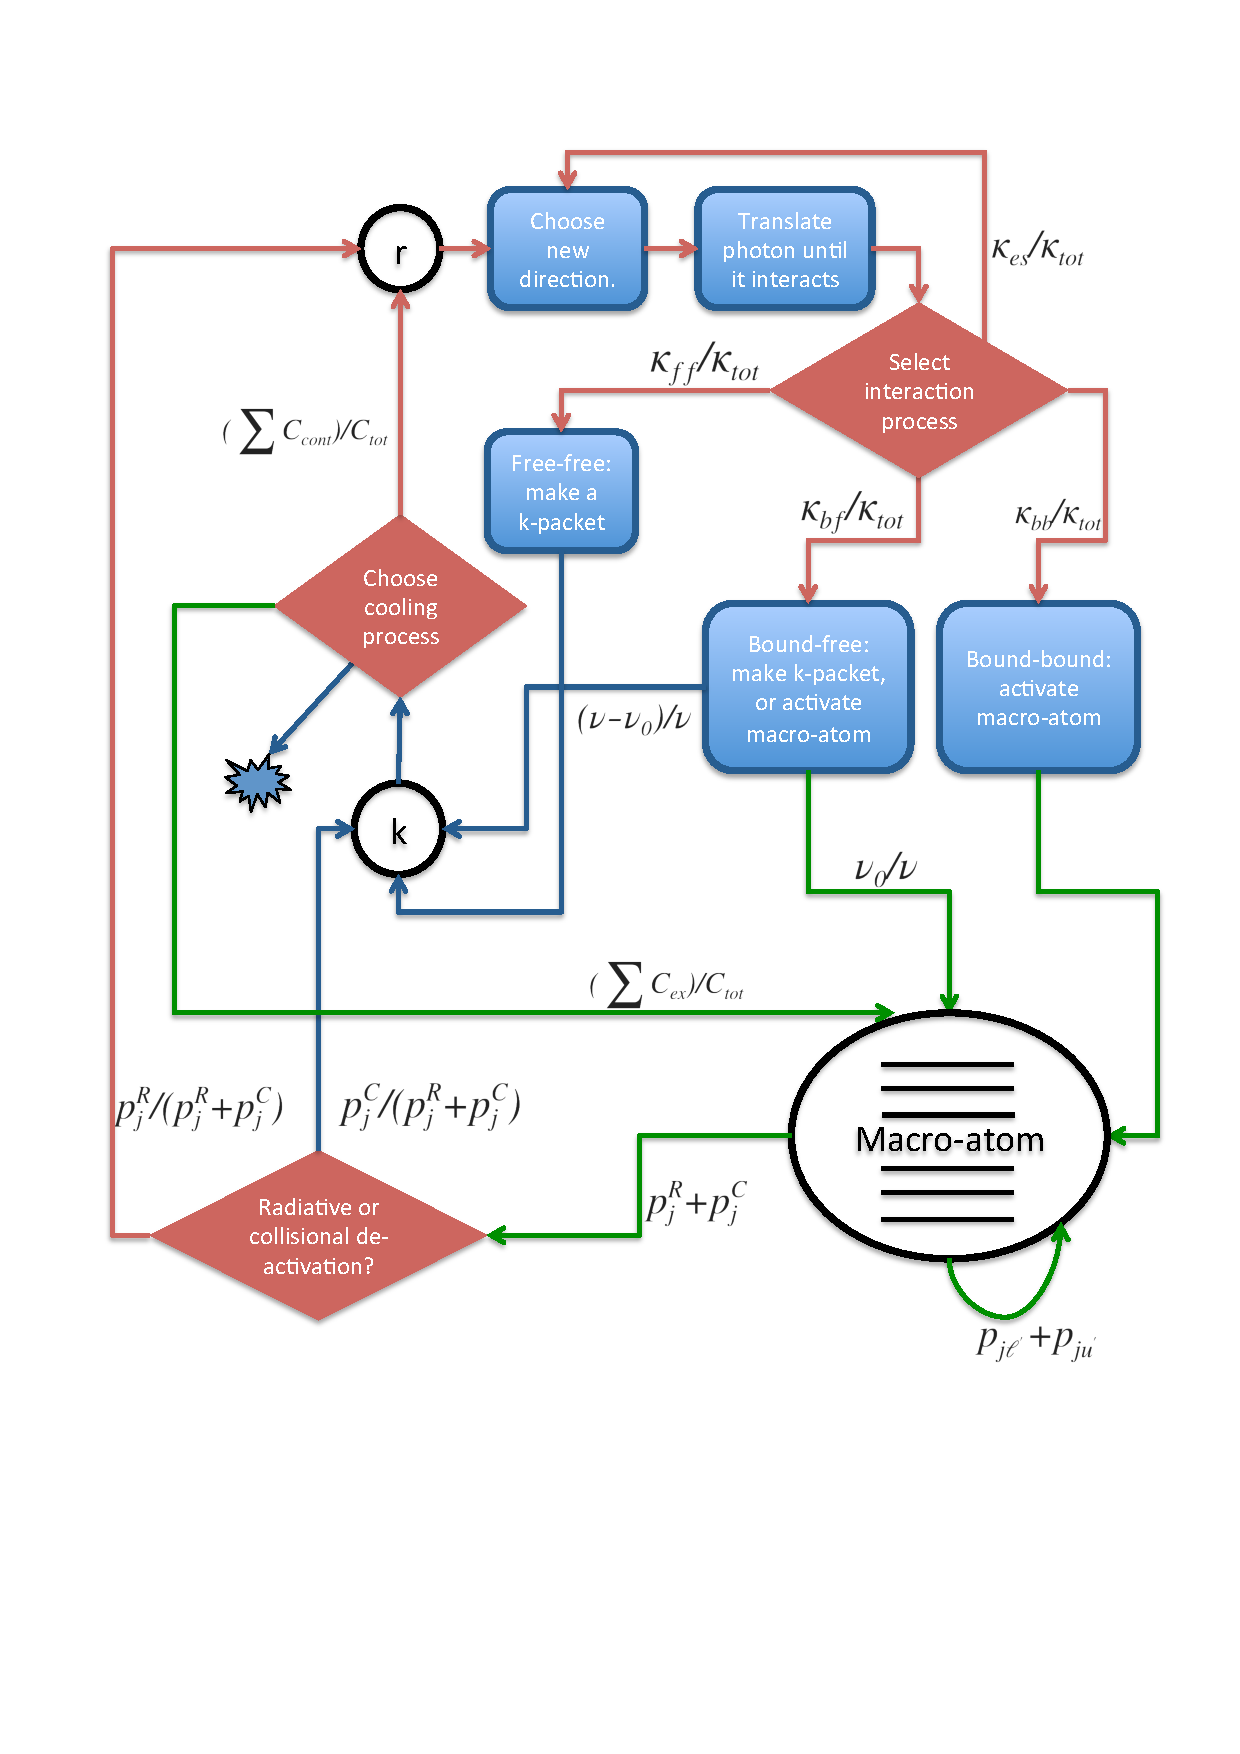
\includegraphics[width=1.0\textwidth, clip=true, trim=0 2.6in 0in 0in ]{figures/03-radtrans/flow_colour.pdf}
\caption
{
The decision tree traversed by an energy packet 
in macro-atom mode, depicting the interaction
between radiation ($r$-packets), the thermal pool ($k$-packets), and ionization
and ionization/excitation energy (macro-atoms). 
The probabilities at each decision point are 
marked, and are defined in the text. The red, blue and green coloured arrows
represent radiant, kinetic and ionization/excitation energy respectively.
} 
\label{fig:flow_matom}
\end{figure}

%% XXX CHECK THIS.


%%%%%%%%%%%%%%%%%%%%%%%%%%%%%
% POPS
%%%%%%%%%%%%%%%%%%%%%%%%%%%%%


\subsection{Ionization Fractions and Level Populations}

In section~\ref{sec:lte} I described how it is possible to calculate the
ionization and excitation of a plasma under LTE or dilute approximations.
Macro-atoms are not approximated -- their level and ion populations are 
calculated by solving the rate equations formulated in section~??. 
This is done via matrix inversion. For an element with $n$ ions and $m_i$
levels in each ion, we construct a square matrix with dimensions 
$m = \sum_i^n m_i$.
This element then has a total number density of $N_{elem} = \sum_i^n N_i$.
To turn the system of rate equations for this element into matrix form, we
populate the $j$th diagonal of the matrix with the negative of the rate out of
level $j$, $-({\cal R}_{j\ellp} + {\cal R}_{j\up})$, 
and populate the off-diagonals $(j,k)$ with the positive rate 
${\cal R}_{jk}$. These are then multiplied by a vector of the fractional level
populations, and must equal a vector of zeros, due to statistical equilibrium.
Our matrix equation is then
%
\begin{equation}
\begin{bmatrix}
    -{\cal R}_{1\up} & {\cal R}_{21} & {\cal R}_{31} & \dots & {\cal R}_{m1} \\
    {\cal R}_{12} & -({\cal R}_{2\ellp} + {\cal R}_{2\up}) & {\cal R}_{32} & \dots & {\cal R}_{m2} \\
    {\cal R}_{13}  & {\cal R}_{23} & -({\cal R}_{3\ellp} + {\cal R}_{3\up}) & \dots & {\cal R}_{m3} \\
    \vdots & \vdots & \vdots & \ddots & \vdots \\
    {\cal R}_{1m}      & {\cal R}_{2m} & {\cal R}_{3m} & \dots & -{\cal R}_{m\ellp}
\end{bmatrix}
\begin{bmatrix}
    n_1 / N_{elem} \\
    n_2 / N_{elem} \\
    n_3 / N_{elem} \\
    \vdots         \\
    n_m / N_{elem} 
\end{bmatrix}
=
\begin{bmatrix}
    0 \\
    0 \\
    0 \\
    \vdots \\
    0
\end{bmatrix}
.
\end{equation}
%
This problem is not yet soluble, as a valid solution is that all levels 
could simply have occupation numbers of $0$. To close the problem, we must impose the boundary condition, that the sum of the fractional populations is 1, i.e.
%
\begin{equation}
\sum_i \frac{N_i}{N_{elem}} = 1.
\end{equation}
In matrix form, this is equivalent to replacing the entire first row
of the rate matrix with 1, and the first entry of the RHS vector with a 1,
so that we have
%
\begin{equation}
\begin{bmatrix}
    1  & 1 & 1 & \dots & 1\\
    {\cal R}_{12} & -({\cal R}_{2\ellp} + {\cal R}_{2\up}) & {\cal R}_{32} & \dots & {\cal R}_{m2} \\
    {\cal R}_{13}  & {\cal R}_{23} & -({\cal R}_{3\ellp} + {\cal R}_{3\up}) & \dots & {\cal R}_{m3} \\
    \vdots & \vdots & \vdots & \ddots & \vdots \\
    {\cal R}_{1m}      & {\cal R}_{2m} & {\cal R}_{3m} & \dots & -{\cal R}_{m\ellp}
\end{bmatrix}
\begin{bmatrix}
    n_1 \\
    n_2 \\
    n_3 \\
    \vdots \\
    n_m
\end{bmatrix}
=
\begin{bmatrix}
    1 \\
    0 \\
    0 \\
    \vdots \\
    0
\end{bmatrix}
\end{equation}
%
This matrix equation can now be solved.
To do the actual matrix manipulation, the code uses the GNU 
scientific libraries \citep[GSL;][]{GSL} implementation of
LU decomposition \citep{turing}. This is a fast and reliable way of
inverting large matrices that includes error handling and enables
checking of, for example, singular rate matrices.














%%%%%%%%%%%%%%%%%%%%%%%%%%%%%
%SIMPLE ATOMS
%%%%%%%%%%%%%%%%%%%%%%%%%%%%%

\section{A hybrid line transfer scheme: including simple-atoms}

I have now described in detail how the macro-atom approach is 
implemented in \py. A pure macro-atom approach can be easily used for
some situations -- for example, in the YSO application described by 
\cite{simmacro2005}, which uses a H-only model. However, in accretion
disc winds the densities can be very high and higher $Z$ elements must be 
included. To include all these elements as macro-atoms is not
currently computationally feasible in \py\ for anything but the simplest
models. I will thus describe a `hybrid scheme', which treats H and He
under the macro-atom approach but models all other atoms 
as `simple-atoms'. 

\subsection{Line Transfer}

Simple-atoms still interact with $r$- and $k$-packets,
but do not possess internal transition probabilities. As a result,
they are analogous to the two-level atom treatment, as any excitation
is immediately followed by a deactivation into an $r$- or $k$-packet.
This hybrid approach allows us to preserve the fast treatment 
of, for example, UV resonance lines, while accurately 
modelling the recombination cascades that populate the levels 
responsible for H and He line emission. As a result of this hybrid
scheme, a separate set of estimators must be recorded for simple-atoms, 
and the ionization and excitation of these elements is calculated 
with a different, approximate approach.

In order to include simple-atoms, we must add in a few extra pathways
to Fig.~\ref{fig:flow_matom}, so that energy packets can also
undergo excite simple-atoms, through either bound-free or bound-bound
processes. This is done in proportion with the simple-atom opacities.

This approach does necessitate a few approximations.

\subsection{Heating and Cooling Estimators}
In simple-ions it is in some ways a little more complicated. 
First we define $q$ which will be different for each b-b transition, 
following Nick's thesis, which is given by 
(NB: I don't actually know how to derive this)
\begin{equation}
q = \frac{q_{ul} n_e (1 - e^{-h\nu/kT_e})}{\beta_{ul} A_{ul} + q_{ul} n_e (1 - e^{-h\nu/kT_e})}
\end{equation}
where $\beta_{ul}$ is the angle-averaged escape probability. 
$q$ represents {\em the probability that an excited bound electron
will collisionally de-excite}.
Our b-b heating rate is computed during the photon propagation and is a sum
over photons which come into resonance with each line, given by 
\begin{equation}
H_{bb,simple} = \sum_{photons} \sum_{lines} (1 - q) (1 - e^{-\tau_S}) w_{photon}
\end{equation}
And our bound bound cooling rate is given by 
\begin{equation}
C_{bb,simple} = \sum_{lines} q \left(n_l\frac{g_u}{g_l} - n_u\right) q_{ul} n_e 
\frac{(1 - e^{-h\nu/kT_e})}{(e^{h\nu/kT_e} - 1)}  h \nu_{ul}
\end{equation}
%%note the difference to the macro-atom approach- here this is already 
\noindent
The bound-free heating rate is given by
\begin{equation}
H_{bf,simple} = \sum_{photons} \sum_{bfjumps} w_{photon} e^{-\tau} \frac{\nu - \nu_{0}}{\nu}
\end{equation}
where $\nu$ here is the frequency of the photon in question, and $\nu_{0}$.
The bound-free cooling rate is then
\begin{equation}
C_{bf,simple} = ??
%%\sum_{bfjumps} \alpha_{sp} n_e n_{\kappa}
\end{equation}

\subsubsection{Radiation Field Estimators}

For simple-atoms we do not record radiation field estimators for discrete 
transitions, as for macro-atoms. Instead, we record estimators to
give us a model of the radiation field. The estimators needed
depend on the ionization mode employed (see section~\ref{sec:simple_ionization}).
The radiation temperature, $T_R$, is estimated by recorded the mean frequency, 
$\bar{\nu}$, of the photons passing through a cell:
\begin{equation}
\bar{\nu} = \frac{\sum_{photons} w_i \nu_i \Delta s}{\sum_{photons} w_i \Delta s}.
%%\sum_{bfjumps} \alpha_{sp} n_e n_{\kappa}
\end{equation}
This is then used to calculate the radiation temperature by
considering the value expected from a blackbody \cite{ML93}, giving 
\begin{equation}
T_r = \frac{h\bar{\nu}}{3.832~k}
\end{equation}
The dilution factor can be calculated by comparing the estimator for the mean intensity 
to the Stefan-Boltzmann law:
\begin{equation}
W = \frac{\pi J}{\sigma~T_r^4}.
\end{equation}
This set of estimators is sufficient to describe the 
radiation field if one is adopting the dilute approximation (section~\ref{sec:dilute}).
\cite{higginbottom2013} improved on this by developing a method for
modelling the SED in the cell using a series of band-limited 
radiation field estimators. In this scheme, a series of bands is defined
in which to record these estimators. These bands are different to the bands
discussed in section~\ref{sec:packets} as those instead govern photon generation.
In H13, the band limited estimators were used to construct a correction factor
that could be used in a modified Saha equation 
(similar in form to equation~\ref{eq:ml93}). However, the code has now been
improved so that the ion populations are computed by solving the rate equations.
Thus, we now simply need to calculate photoionization rate estimators for simple 
ions, which rely on being able to integrate a modelled form of the mean intensity.



\subsection{Ionization and Excitation}
\label{sec:simple_ionization}


% Prior to SDL05, the relative ionization fractions for all atomic
% species were estimated via the modified Saha equation (Mazzali \&
% Lucy 1993)  
% \begin{equation}
% \frac{n_{j+1} n_e}{n_j} = W [\xi + W(1-\xi)]
% \left(\frac{T_e}{T_R}\right)^{1/2}
% \left(\frac{n_{j+1}n_e}{n_j}\right)^*_{T_R}. \label{ionization}
% \end{equation}
% Here, the `starred' term on the right represents abundances computed with
% the Saha equation at temperature $T_R$, but using partition functions
% from the dilute blackbody approximation. 
% $W$ is an effective dilution factor, $\xi$ is the
% fraction of recombinations going directly to the ground state, and
% $T_R$ and $T_e$ are the radiation and electron temperatures,
% respectively. This simple ionization scheme produces reasonable
% results when the photoionizing SED can be approximated by a dilute
% blackbody. This is the case for high-state CVs. (As noted above, an
% improved, but more complex treatment of ionization that is appropriate
% for more complex SEDs is described in H13.) 

Regardless of ion mode, the relative excitation fractions of simple-atoms
within each ionization stage of a given species are estimated via a modified (dilute) Boltzmann
equation (equation~\ref{eq:dilute_boltzmann}). This equation is approximate, and in 
general this approximation is not good. We therefore endeavour to treat any species in
which the excitation state of the ions is thought to be important
in determining either the ionizing radiation field, or emergent spectrum,
as macro-atoms.

% Finally, \py\ originally modelled all bound-bound processes as transitions
% within a simple two-level atom \cite[e.g.][]{mihalas}. 
% This framework was used for the treatment of line transfer and also
% for the line heating and cooling calculations (see LK02). 
% The approximation works reasonably well for resonance  
% lines, such as \civfull, in which the lower level is the ground state.  
% However, it is a poor approximation for many other
% transitions, particularly those where the upper level
% is primarily populated from above. Thus an improved method for
% estimating excited level populations and simulating line transfer is
% needed in order to model recombination lines and continua.

\section{Heating And Cooling Balance}
\label{sec:heating_cooling}
I have already given the estimators used to calculate
heating and cooling rates in the plasma. These are not only used
in the creation and elimination of $k$-packets, but also in the heating
and cooling balance carried out in \py\ to achieve a self-consistent
temperature structure in the wind. 

At the end of each ionization cycle, the code has stored a new set
of MC estimators for radiative heating of the plasma. We then
assume that each cell is in thermal equilibrium then the appropriate
electron temperature is simply the value of $T_e$ that is a solution
to the equation
\begin{equation}
\hh_{tot} - \cc_{tot} ( T_e) = 0,
%%\sum_{bfjumps} \alpha_{sp} n_e n_{\kappa}
\end{equation}
where $\hh_{tot}$ and $\cc_{tot}$ are the total heating and cooling rates in 
the plasma. A number of checks are in place to ensure numerical stability,
namely a maximum temperature and a maximum change in temperature from cycle
to cycle. This is especially important in cases where the initial
guess at wind temperature is far from the true value.

\subsection{Convergence}

\py\ always runs a fixed number of ionization cycles, rather than terminating
when a convergence criterion is reached. As a result, it is up to the user
to check that the simulation is converged. An individual cell is considered
converged when a) the temperature stops changing signicantly, i.e. both
$T_R$ and $T_e$ satisfy
\begin{equation}
\frac{|T_{new} - T_{old}|}{T_{new} + T_{old}} < 0.05,
%%\sum_{bfjumps} \alpha_{sp} n_e n_{\kappa}
\end{equation}
and b) the heating and cooling rates are well balanced such that
\begin{equation}
\frac{|\hh_{tot} - \cc_{tot}|}{\hh_{tot} + \cc_{tot}} < 0.05.
%%\sum_{bfjumps} \alpha_{sp} n_e n_{\kappa}
\end{equation}
These criteria could doubtless be improved, but they are nonetheless
a good way of ensuring that thermal and radiative equilibrium holds in the 
plasma. An example of how the average temperature and fraction
of converged cells changes over the course of the ionization cycles in
a typical CV model is shown in Fig.~\ref{fig:conv}.


\begin{figure}
\centering
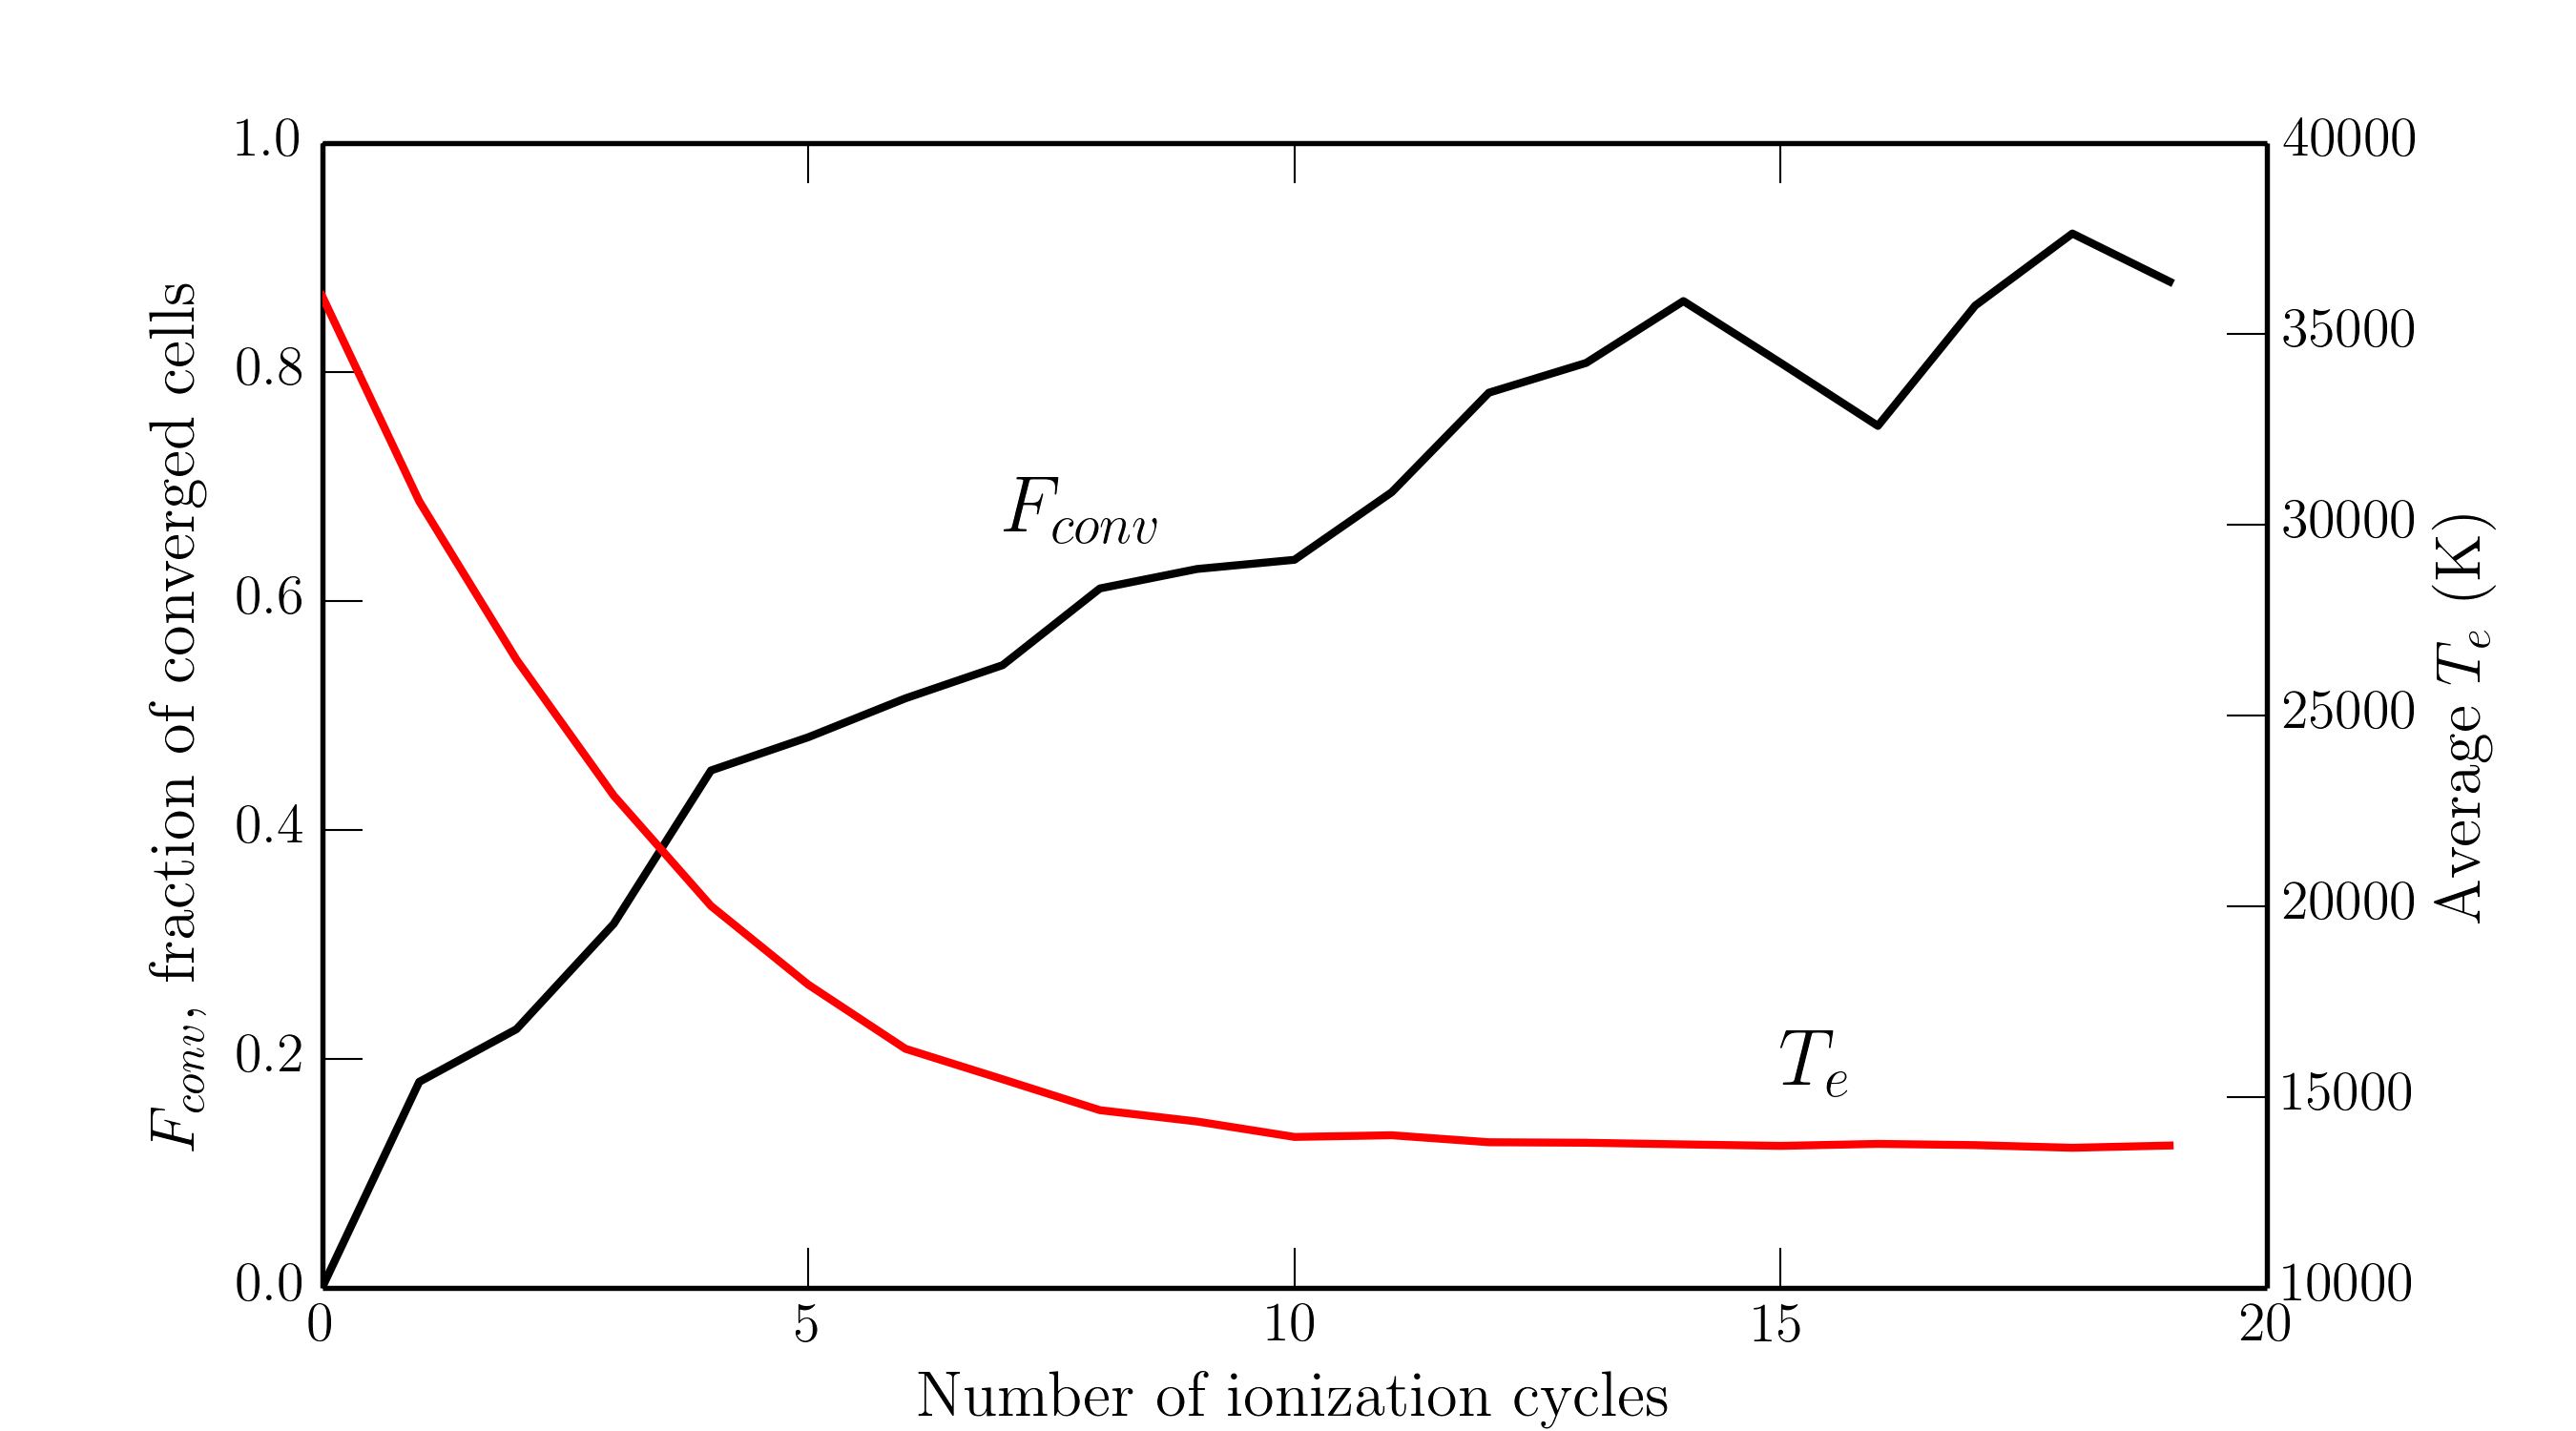
\includegraphics[width=1.0\textwidth]{figures/03-radtrans/graph_conv.png}
\caption
{
The average temperature and fraction of converged cells in
a typical CV model, shown as a function of the number of ionization cycles
completed. 
} 
\label{fig:conv}
\end{figure}




\section{Spectral Cycles}
\label{sec:spectral_cycles}
The primary output from \py\ is a synthetic spectrum 
across a range of viewing angles. The code utilises a variance 
reduction technique in order to minimise the amount of 
time spent in the portion of the code. This technique is based 
on a similar method implemented by \citep{woods1991}.






A comparison between the two methods is shown in figure~\ref{fig:extract_demo}.

\begin{figure}
\centering
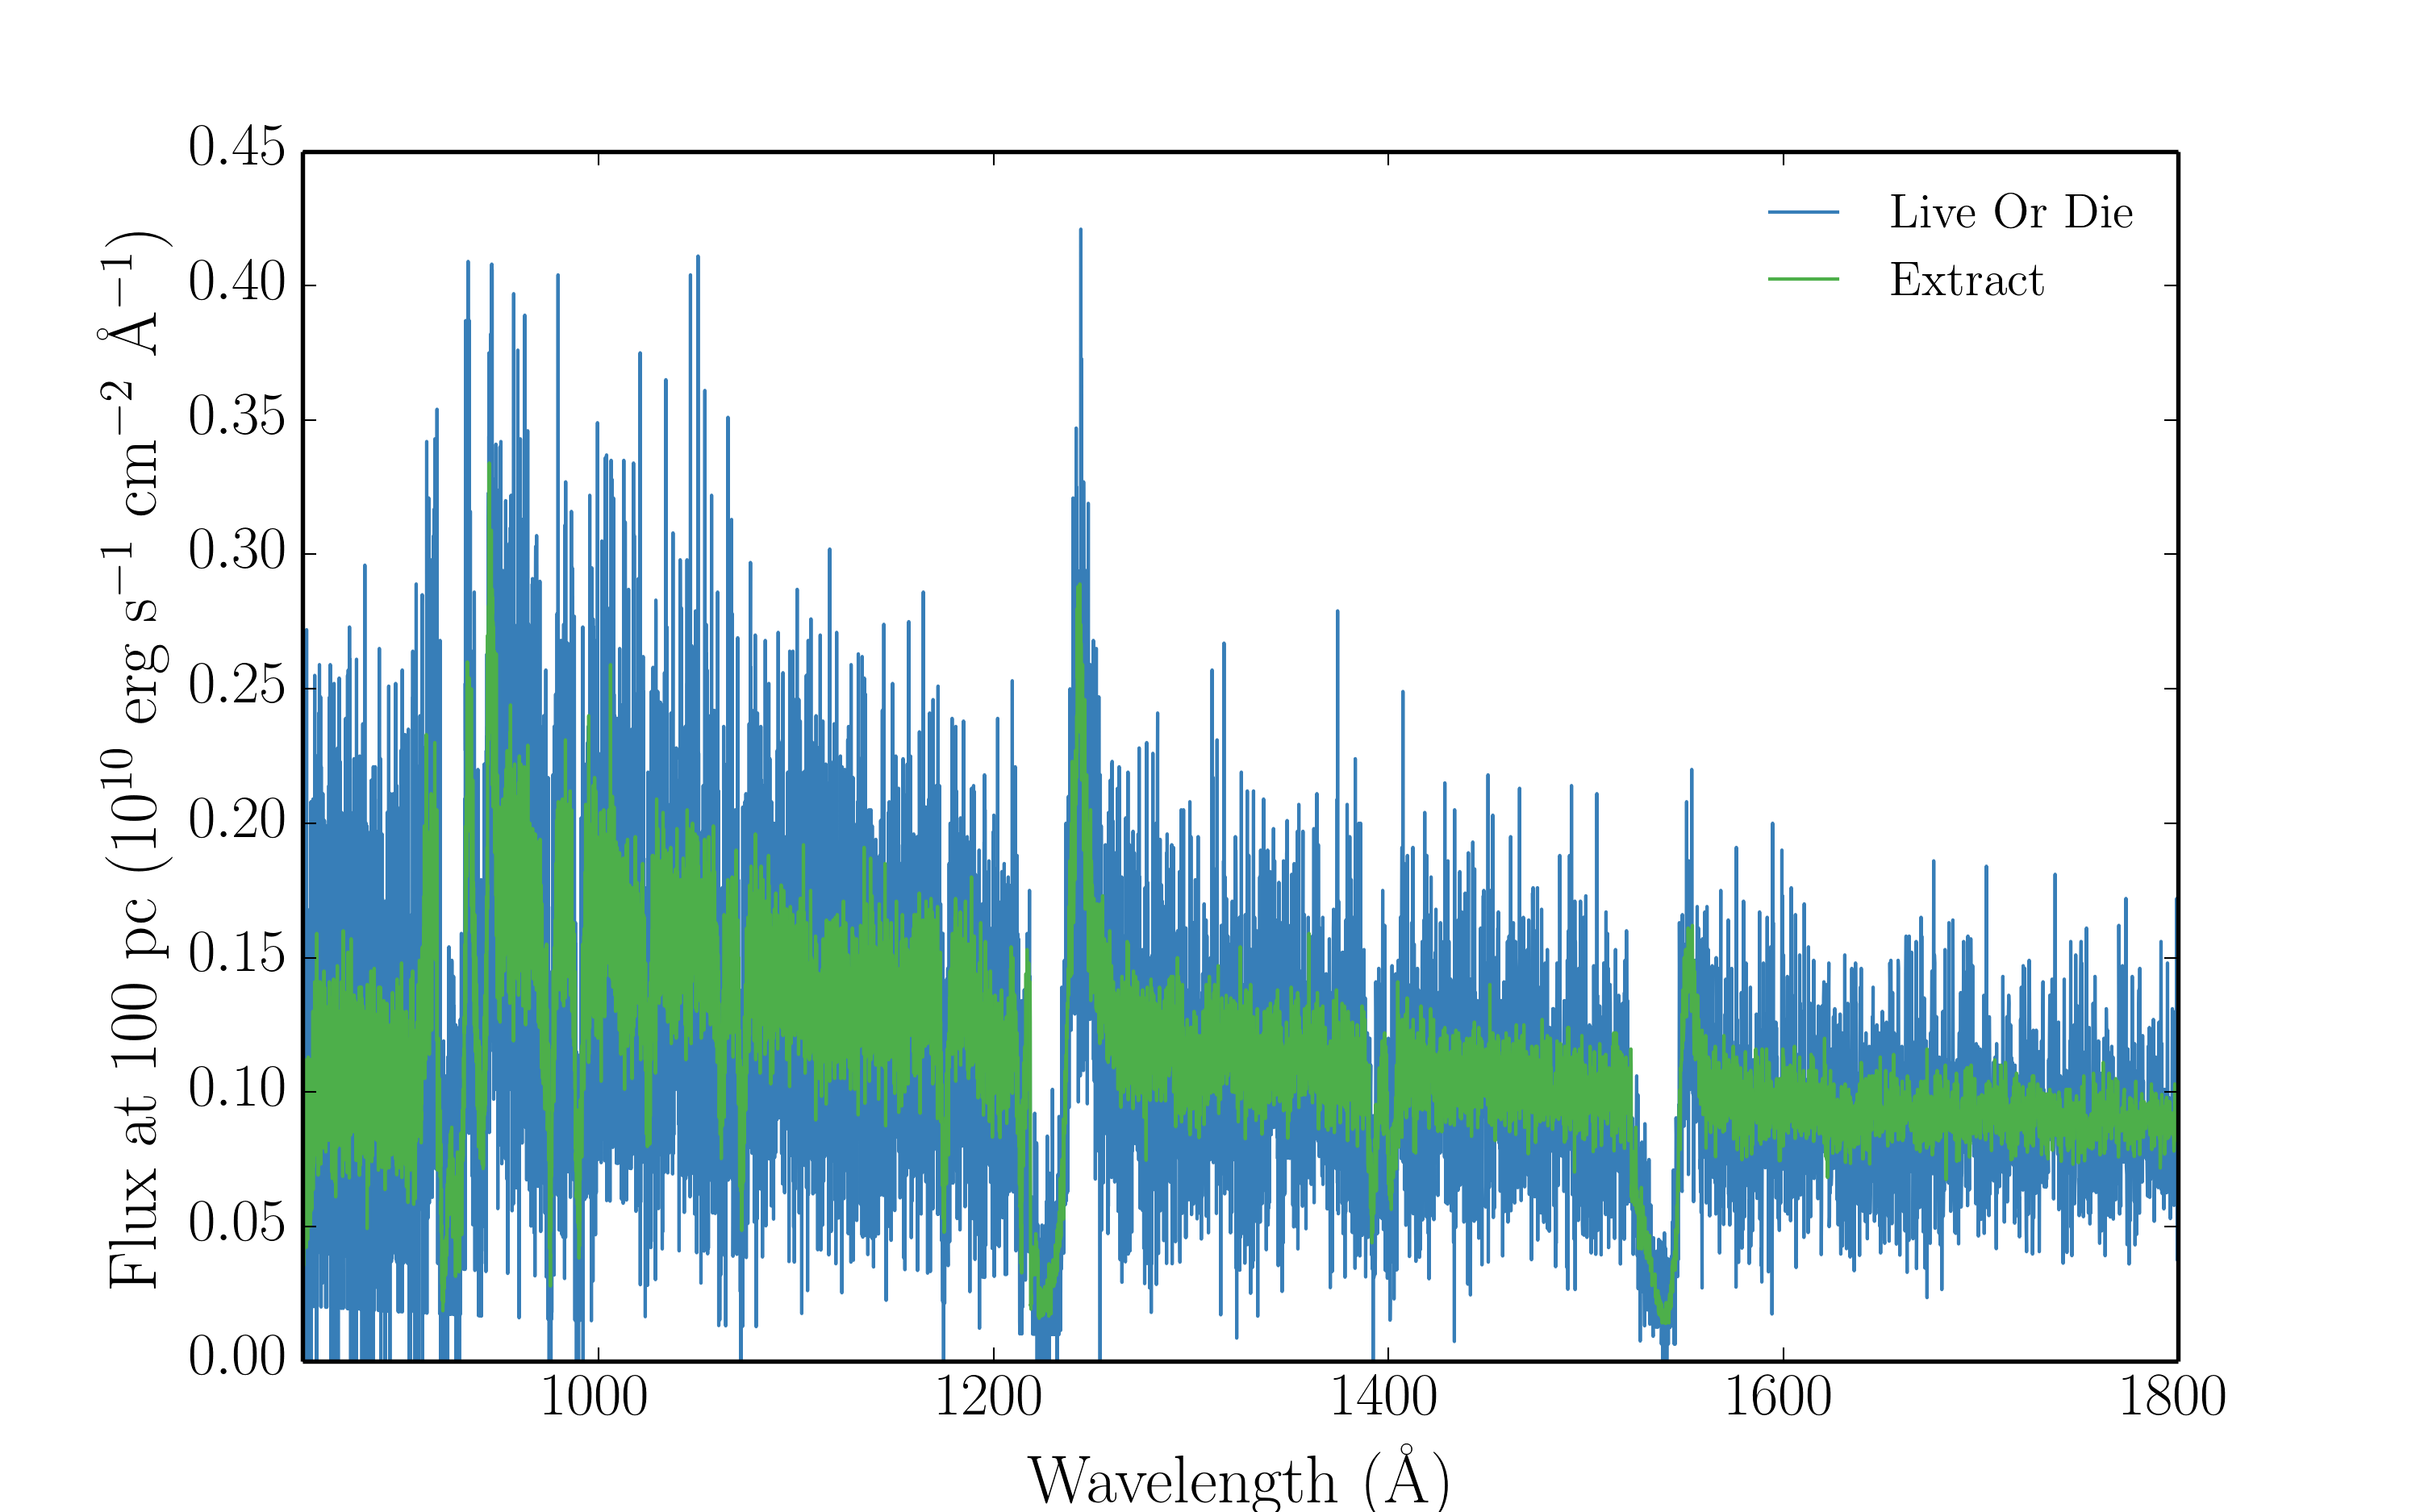
\includegraphics[width=1.0\textwidth]{figures/03-radtrans/extract_demo.png}
\caption
{
A Synthetic spectrum after $30$ spectral cycles with $100,000$ photons
from simple CV wind model at a $60^\circ$ viewing angle.
Spectra produced with both the extract and live or die modes
are shown. The effectiveness of the extract variance reduction technique can
be clearly seen, and we can see that the spectral shape is unaltered.
} 
\label{fig:extract_demo}
\end{figure}




\section{Atomic Data}

One of the big challenges in building reliable photoionization and radiative
transfer lies in the acquisition of accurate and complete atomic datasets.
All of the rates described so far contain a term, such as the oscillator strength 
or dimensionless collision strength, that is dependent purely on the atomic physics
associated with the transition. These quantities can be measured in laboratory experiments,
or predicted from atomic structure codes which derive the atomic physics from 
quantum theory.

Photoionization cross-sections are obtained from two sources. Where possible,
we use \top\ photoionization cross-sections. For macro-atoms,
these cross-sections are partial and represent the cross-section for a photoionization
from a given {\em level}. We neglect photoionizations to excited configurations
of the upper ion. For simple-atoms they are from the ground state.
The \top\ cross-sections have two major drawbacks in that 

In order to improve the \top\ cross-sections, I have extrapolated them to larger
energies. This was done by finding the slope, in log-log space
of the cross-section at the maximum energy, and extrapolating to $100$~keV.
In some cases, the slope near the maximum energy was anomalous 
due to resonances or similar structure in the cross-section, or possibly
simply due to unknown problems in the \top\ calculations. These
cases were identified by eye, and instead a $\nu^{-3}$ extrapolation
was applied. The results of this extrapolation on the H13 model
are shown in figure~\ref{fig:xs}. Where previously there was a sharp,
unphysical edge, we know observe the typical recovery to an X-ray 
power law we expect.

\begin{figure}
\centering
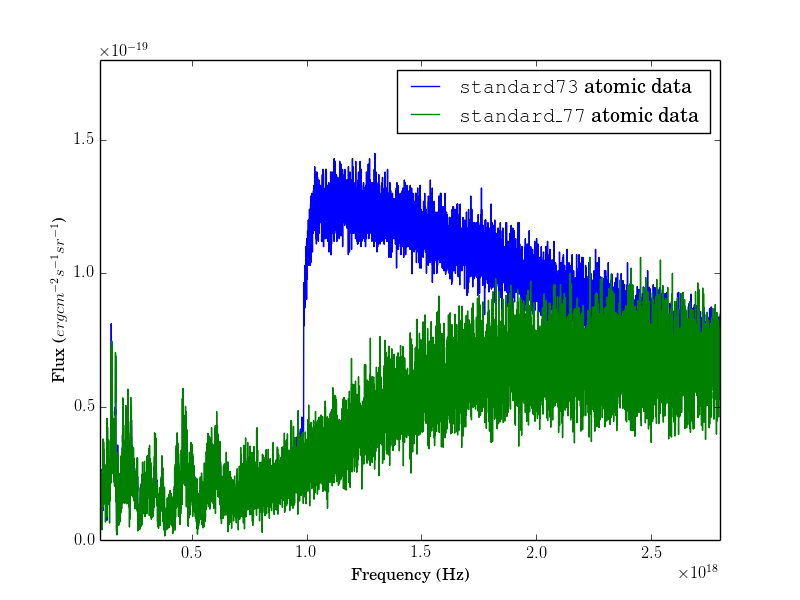
\includegraphics[width=1.0\textwidth]{figures/03-radtrans/xs.png}
\caption{
A comparison of the soft X-ray regime of the H13 model, with two different
datasets. standard73 is the dataset with old, unextrapolated cross-sections 
and standard77 instead includes extrapolated cross-sections as described in
the text.
}
\label{fig:xs}
\end{figure}

% \section{Clumping}

% \label{sec:microclumping}

% \subsection{Motivation}

% As described in section~??, observational evidence for inhomogeneities in 
% outflows is widespread. Clumping a plasma can have a significant effect on its
% ionization, emission and absorption characteristics. Clearly, the interplay between
% these effects will be somewhat complex 

% A number of different implementations of clumping have been explored in previous studies,
% mostly in the stellar winds community. Perhaps the simplest method is 
% when one assumes that the individual clumps are both optically and geometrically thin;
% this is known as {\em microclumping} \citep[e.g.][]{hamann1998,hilliermiller1999,hamann2008}. 
% This technique has been particularly successful in reconciling 
% discrepant mass-loss estimates.
% It was found that one would obtain different mass-loss rates depending on whether
% they were calculated from (i) UV resonance scattering of continuum photons 
% (which scales linearly with density; a `$\rho$-diagnostic') or (ii) recombination 
% and free-free emission process (which scale with the square of density; 
% `$\rho^2$-diagnostics'). A clumped outflow would have enhanced densities in 
% certain regions, and would thus mean that $\rho^2$-diagnostics tend to 
% overestimate the total mass-loss rates. Microclumping has helped verify this
% hypothesis with radiative transfer modelling (REFs). These clumpy models also
% provide better fits to the electron scattering wings of emission lines in stellar
% winds \citep{hillier1991}.

% The second-generation of stellar wind codes went on step further by addressing the issue
% of {\em porosity}; that clumps will have a finite size, and thus gaps between the clumps
% may affect the emergent radiation field. This approach is known as {\em macroclumping}.
% {\bf Describe macroclumping with references.}

% Implementing a treatment of clumping in accretion disc wind models is challenging, for
% two main reasons. First, the physical scale lengths and density contrasts 
% in disc winds are not well-constrained from observations, especially in AGN.  
% Second, there are significant computational difficulties associated with adequately
% resolving and realistically modelling a series of small scale, high density
% regions with a MCRT code. Given the lack of knowledge about the actual 
% type of clumping, we encorporated the simpler microclumping approach into our code.
% This is partly because our primary concern was the ionization and 
% emission characteristics of the flow, and porosity was a secondary concern.


% \subsection{Microclumping}

% To take account of clumping in our outflow we adopt a simple parameterization
% used in stellar wind modelling. The key assumption here is that typical clump sizes
% are much smaller than the typical photon mean free path, and thus the clumps are 
% both geometrically and optically thin. This approach is typically 
% known as microclumping and allows one to introduce a `filling factor', $f$, which is the 
% fraction of the volume of the plasma filled by clumps. We can then introduce the 
% `density enhancement', $D$, which is simply 

% \begin{equation}
% D = \frac{1}{f}
% \end{equation}

% The densities in the model are then multiplied by this factor. This has the effect 
% of enhancing `$\rho^2$' processes such as recombination or collisional excitation,
% and 


\section{Code Validation}
\label{sec:code_validation}

The main challenge for high performance scientific computing can be 
elegantly summarised by Ferland's (2002) epitaph, {\sl `Reliability in the face 
of complexity'}. I have already delved into some of the complexity in this case,
so it is important to assess whether the code is also reliable before I present
results. 

\subsection{Testing against \cld}



\subsection{Macro-atom testing against \tar and theory}

\tar\ is a 1D photoionization and radiative transfer designed to
model SNe in a quick and easy python package, and is described in detail by
\cite{kerzendorfsim}. Although \tar\ is simpler in terms
of geometry, it has many of the same capabilities of \py\ and 
thus makes for an excellent comparison. 

Fig.~\ref{fig:caseb_tests} shows the results of two code tests. 
In the top panel, I show a comparison of the Balmer series 
emissivities as predicted by \py\ in the l-mixed Case~B limit against the
analytical calculations by \cite{seaton1959}. 
Both calculations are calculated at $T_e=10,000$K.
Case B is an approximation commonly used in nebular astrophysics in which
one assumes that all transitions are optically thin, except
for the \la\ transition, which is taken as optically thick.
Thus, this test comparison is carried out using a thin shell
of plasma in which the escape probabilities, $\beta_{ul}$ 
are artificially set to 1 in all transitions except \la, which
has its $\beta_{ul}$ set to 0.

The bottom panel shows a comparison of He I level populations 
(the most complex ion currently 
treated as a macro-atom) between \py\ and \tar models.
The calculation is conducted with physical parameters of $n_e=5.96\times10^4$~cm$^{-3}$,
$T_e=30,600$K, $T_R=43,482$K and $W=9.65\times10^{-5}$. 
Considering the two codes use different atomic data and 
\textsc{Tardis,} unlike \textsc{Python,} currently has a 
complete treatment of collisions between 
radiatively forbidden transitions, the factor of 
$<2$ agreement is encouraging. 

\begin{figure}
\centering
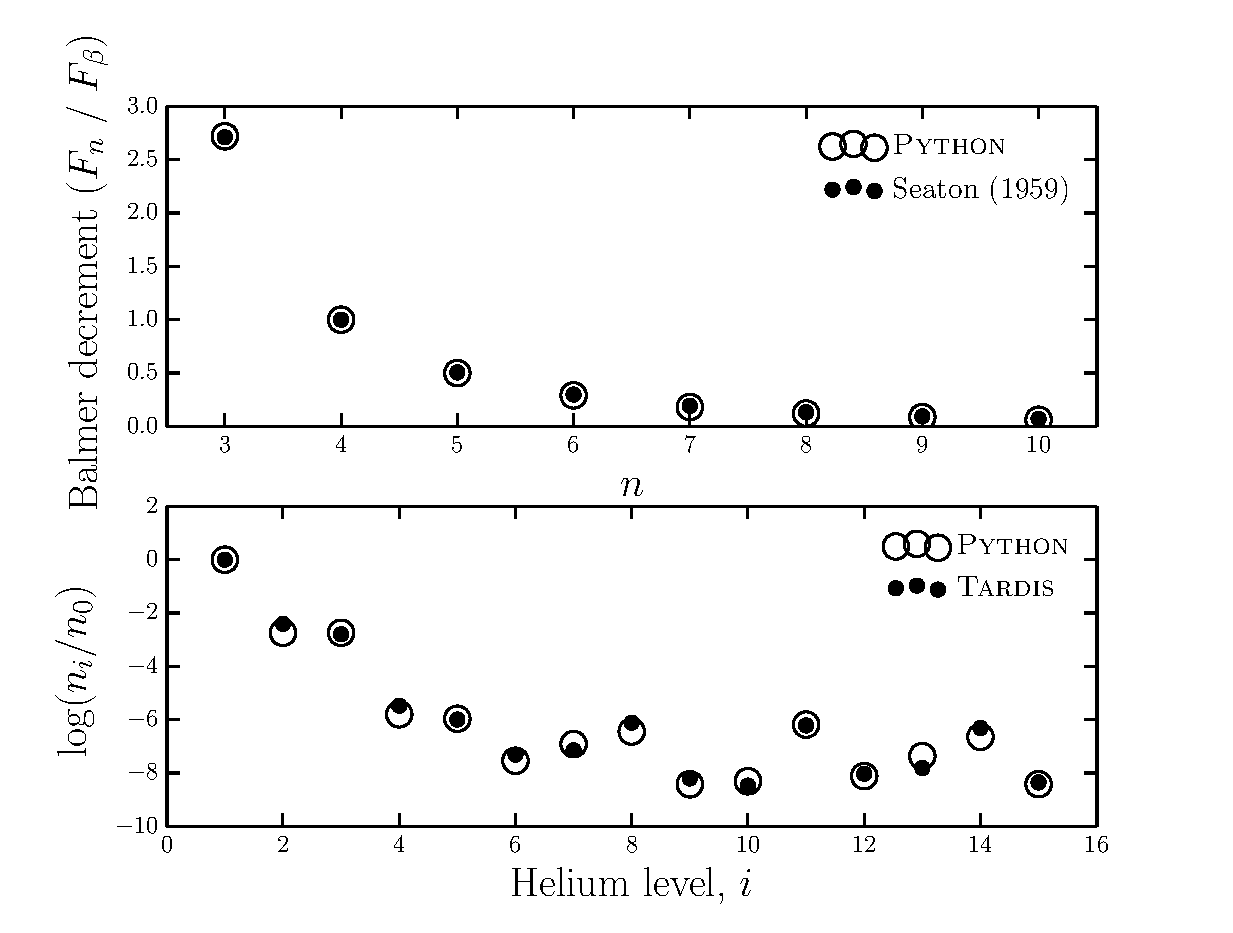
\includegraphics[width=1.0\textwidth]{figures/05-cvpaper/fig_caseb_tardis.eps}
\caption{
{\sl Top Panel:} `Case B' Balmer decrements computed 
with \textsc{Python} compared to analytic calculations
by Seaton (1959). Both calculations are calculated at $T_e=10,000$K.
(see Osterbrock 1989 for a discussion of this commonly used approximation).
{\sl Bottom Panel:}  a comparison of He I level populations (the most complex ion we currently 
treat as a macro-atom) between \py\ and \tar models. 
The calculation is conducted with physical parameters of $n_e=5.96\times10^4$~cm$^{-3}$,
$T_e=30,600$K, $T_R=43,482$K and $W=9.65\times10^{-5}$. 
Considering the two codes use different atomic data and 
\textsc{Tardis,} unlike \textsc{Python,} currently has a 
complete treatment of collisions between 
radiatively forbidden transitions, the factor of 
$<2$ agreement is encouraging. 
}
\label{fig:caseb_tests}
\end{figure}

Fig.~\ref{fig:tardis_spec} shows a comparison 
between \tar\ and \py\ synthetic spectra from 
a simple 1D SN model. The model involves a full 
computation of the ionization state in the ML93 mode, and, although
run in 1D, still tests must of the radiative transfer
machinery of the code. The spectra are in good agreement, considering
there are differences in their excitation treatments and atomic data.
This comparison is also particular encouraging when we consider
that \cite{kerzendorfsim} also show comparisons with other SN codes such
as \textsc{Artis} \citep{kromersim2009}.

\begin{figure}
\centering
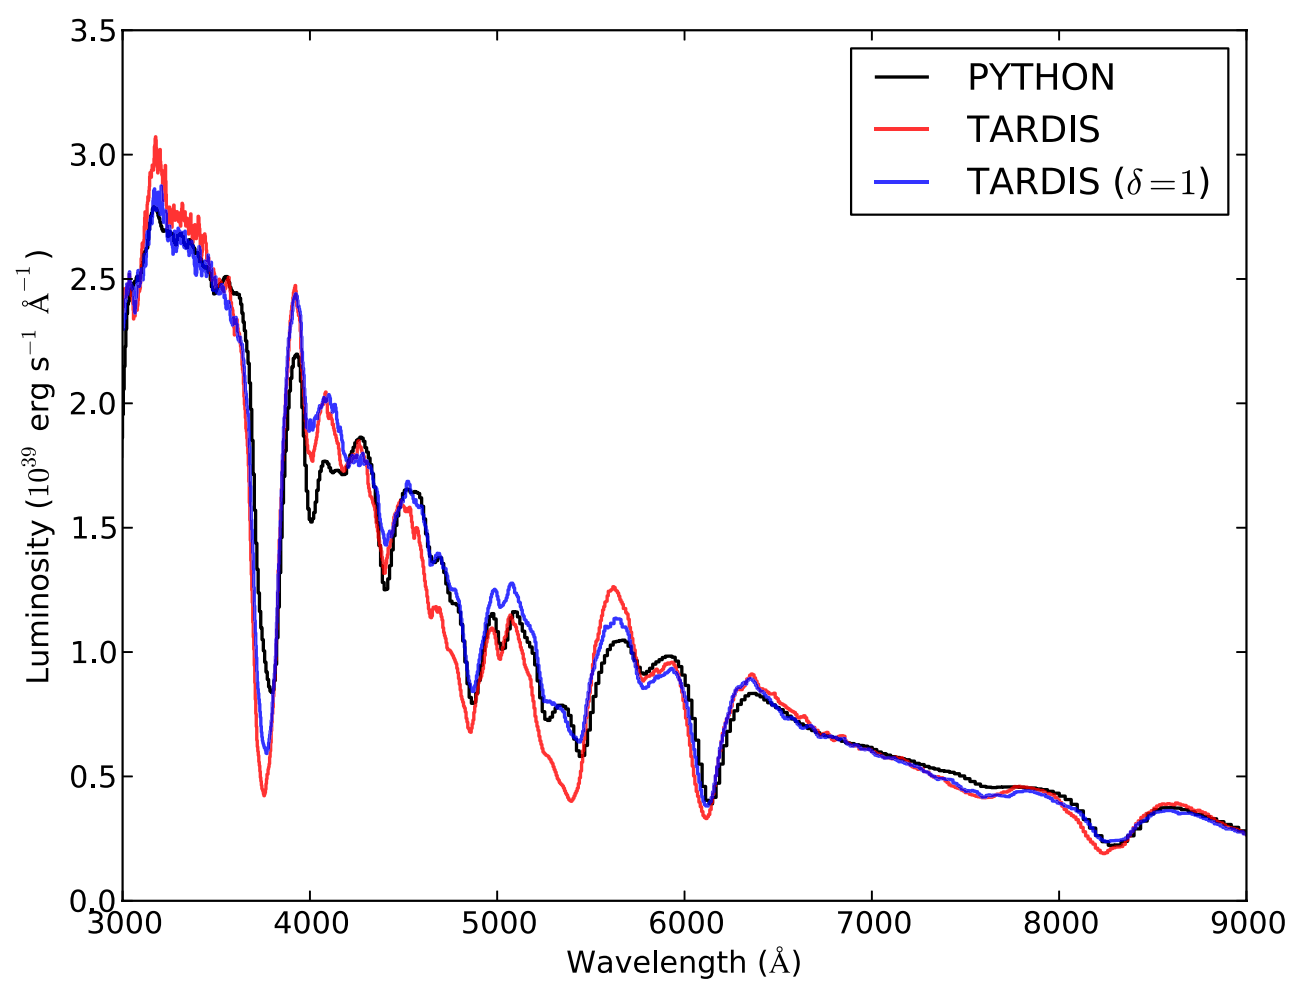
\includegraphics[width=1.0\textwidth]{figures/03-radtrans/tardis_spec.png}
\caption{
{\sl Credit: Kerzendorf \& Sim 2014}.
Comparison between \tar\ and \py\ synthetic spectra from 
a simple 1D supernova model.
$\delta$ is an additional parameter that can be included in the ML93 equation,
and thus the appropriate comparison here is with the $\delta=1$ case.
}
\label{fig:tardis_spec}
\end{figure}

\subsection{Testing line transfer modes}

Include a test of simple ion v standard mode...

\section{Code Maintenance and Version Control}
\label{sec:code_maintenance}

As part of the expansion of the team working on \py\, I was responsible
for bringing the code under the auspices of a robust version control system.
Thanks to these efforts, the code is now hosted on GitHub at 
\url{https://github.com/agnwinds/python/}. Our team uses a Pull \& Fork model
for collaborative code development, in which major changes are made in a 
forked repository before the developer submits a `Pull request' to the main 
repository. To test the code, we use a combination of Travis CI build tests 
-- run per commit to the upstream repo -- and our own test suite which is 
run every night on a multi-core server. 

\begin{figure}
\centering
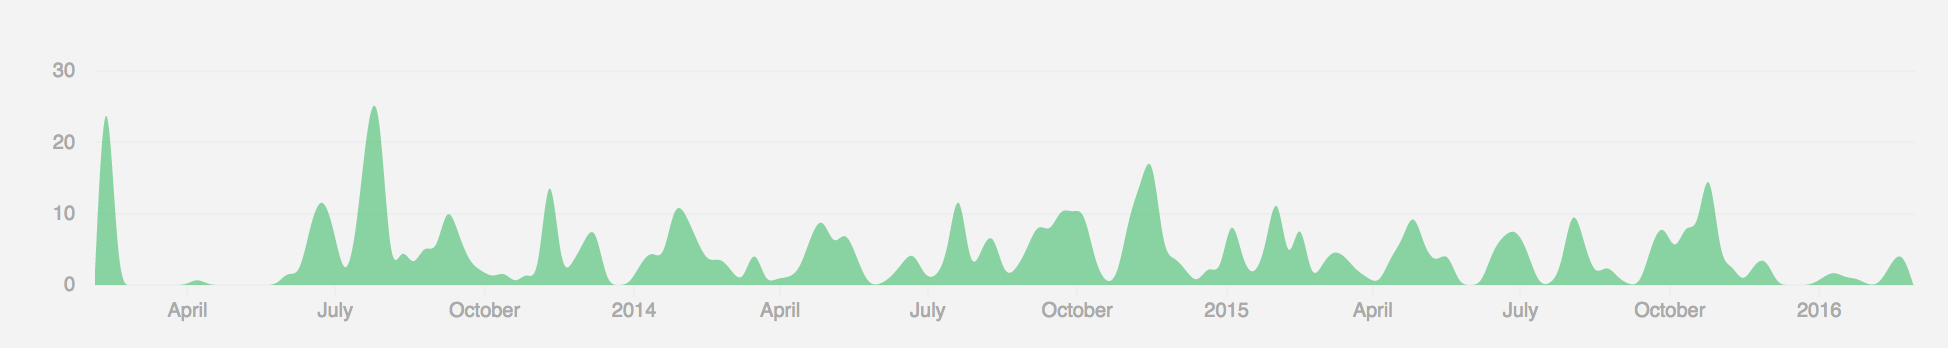
\includegraphics[width=1.0\textwidth]{figures/03-radtrans/github1.png}
\caption
{
Commit history from Feb 3, 2013 to Feb 29, 2016, showing the regular code development
that makes version control such a necessity to a collaborative code project. Produced
using the Github API and plotting capability.
} 
\label{fig:github}
\end{figure}

\subsection{Parallelisation} 

Including macro-atoms in a simulation can have a significant impact 
on runtime, especially when simulating dense regions of plasma. 
By way of example, the CV model presented by LK02 takes approximately
??s to produce a converged model and output spectrum. The model
presented in chapter 4 takes ??s for the same number of cycles and 
photon numbers. 

Fortunately, MCRT codes are intuitively parallelisable, as is the macro-atom
emissivity calculation described above. \py\ is parallelised using an open 
source Message Passing Interface (MPI) implementation known as 
Open MPI \citep{openmpi}. This library provides the core functions needed
in order to distribute computing tasks among a series of parallel processors
with distributed memory. The parallelised elements of \py\ include
the photon propagation, updating of wind ionization and temperature structure
and calculation of macro-atom emissivities. As a result, this involves
a reasonable amount of book-keeping in that the radiation field estimators 
must be communicated between threads so as to correctly account for all
the photons that have interacted with a given cell.

Fig.~?? shows the effect of parallelising a run. Due to the nature of MCRT,
it is possible to achieve a roughly linear decrease in computing time
for the photon propagation, which is the dominant factor in overall 
runtime.



% \section{My Contribution}

% The code and techniques described represent a large collaborative effort
% by a number of different people. It is therefore important to clearly
% identify my specific contribution to the above work.

% \begin{itemize}
% 	\item Parallelisation of the macro-atom estimators (so they are correctly communicated between threads), and the emissivity calculation described in section~??.
% 	\item Improvement of photoionization cross-sections as described in section~??.
% 	\item Incorporation of Helium macro-atom atomic data.
% 	\item Tabulation of VFKY photoionization cross-sections to avoid on the fly calculations
% 	from the fitting formulae.  
% \end{itemize}







